% Options for packages loaded elsewhere
\PassOptionsToPackage{unicode}{hyperref}
\PassOptionsToPackage{hyphens}{url}
\PassOptionsToPackage{dvipsnames,svgnames,x11names}{xcolor}
\documentclass[
  spanish,
  11pt,
  a4paper,
]{article}
\usepackage{xcolor}
\usepackage{microtype}
\usepackage[margin=1in]{geometry}
\usepackage{amsmath,amssymb}
\setcounter{secnumdepth}{-\maxdimen} % remove section numbering
\usepackage{iftex}
\ifPDFTeX
  \usepackage[T1]{fontenc}
  \usepackage[utf8]{inputenc}
  \usepackage{textcomp} % provide euro and other symbols
\else % if luatex or xetex
  \usepackage{unicode-math} % this also loads fontspec
  \defaultfontfeatures{Scale=MatchLowercase}
  \defaultfontfeatures[\rmfamily]{Ligatures=TeX,Scale=1}
\setmonofont{Cascadia Mono}
\fi
\usepackage{lmodern}
\ifPDFTeX\else\setmonofont{Cascadia Mono}\fi
\ifPDFTeX\else
  % xetex/luatex font selection
\fi
% Use upquote if available, for straight quotes in verbatim environments
\IfFileExists{upquote.sty}{\usepackage{upquote}}{}
\IfFileExists{microtype.sty}{% use microtype if available
  \usepackage[]{microtype}
  \UseMicrotypeSet[protrusion]{basicmath} % disable protrusion for tt fonts
}{}
\makeatletter
\@ifundefined{KOMAClassName}{% if non-KOMA class
  \IfFileExists{parskip.sty}{%
    \usepackage{parskip}
  }{% else
    \setlength{\parindent}{0pt}
    \setlength{\parskip}{6pt plus 2pt minus 1pt}}
}{% if KOMA class
  \KOMAoptions{parskip=half}}
\makeatother
\usepackage{color}
\usepackage{fancyvrb}
\usepackage{fvextra}
\usepackage[htt]{hyphenat}
\newcommand{\VerbBar}{|}
\newcommand{\VERB}{\Verb[commandchars=\\\{\}]}
\DefineVerbatimEnvironment{Highlighting}{Verbatim}{commandchars=\\\{\},breaklines=true,breakanywhere=true,fontsize=\small}
% Add ',fontsize=\small' for more characters per line
\newenvironment{Shaded}{}{}
\newcommand{\AlertTok}[1]{\textcolor[rgb]{1.00,0.00,0.00}{\textbf{#1}}}
\newcommand{\AnnotationTok}[1]{\textcolor[rgb]{0.38,0.63,0.69}{\textbf{\textit{#1}}}}
\newcommand{\AttributeTok}[1]{\textcolor[rgb]{0.49,0.56,0.16}{#1}}
\newcommand{\BaseNTok}[1]{\textcolor[rgb]{0.25,0.63,0.44}{#1}}
\newcommand{\BuiltInTok}[1]{\textcolor[rgb]{0.00,0.50,0.00}{#1}}
\newcommand{\CharTok}[1]{\textcolor[rgb]{0.25,0.44,0.63}{#1}}
\newcommand{\CommentTok}[1]{\textcolor[rgb]{0.38,0.63,0.69}{\textit{#1}}}
\newcommand{\CommentVarTok}[1]{\textcolor[rgb]{0.38,0.63,0.69}{\textbf{\textit{#1}}}}
\newcommand{\ConstantTok}[1]{\textcolor[rgb]{0.53,0.00,0.00}{#1}}
\newcommand{\ControlFlowTok}[1]{\textcolor[rgb]{0.00,0.44,0.13}{\textbf{#1}}}
\newcommand{\DataTypeTok}[1]{\textcolor[rgb]{0.56,0.13,0.00}{#1}}
\newcommand{\DecValTok}[1]{\textcolor[rgb]{0.25,0.63,0.44}{#1}}
\newcommand{\DocumentationTok}[1]{\textcolor[rgb]{0.73,0.13,0.13}{\textit{#1}}}
\newcommand{\ErrorTok}[1]{\textcolor[rgb]{1.00,0.00,0.00}{\textbf{#1}}}
\newcommand{\ExtensionTok}[1]{#1}
\newcommand{\FloatTok}[1]{\textcolor[rgb]{0.25,0.63,0.44}{#1}}
\newcommand{\FunctionTok}[1]{\textcolor[rgb]{0.02,0.16,0.49}{#1}}
\newcommand{\ImportTok}[1]{\textcolor[rgb]{0.00,0.50,0.00}{\textbf{#1}}}
\newcommand{\InformationTok}[1]{\textcolor[rgb]{0.38,0.63,0.69}{\textbf{\textit{#1}}}}
\newcommand{\KeywordTok}[1]{\textcolor[rgb]{0.00,0.44,0.13}{\textbf{#1}}}
\newcommand{\NormalTok}[1]{#1}
\newcommand{\OperatorTok}[1]{\textcolor[rgb]{0.40,0.40,0.40}{#1}}
\newcommand{\OtherTok}[1]{\textcolor[rgb]{0.00,0.44,0.13}{#1}}
\newcommand{\PreprocessorTok}[1]{\textcolor[rgb]{0.74,0.48,0.00}{#1}}
\newcommand{\RegionMarkerTok}[1]{#1}
\newcommand{\SpecialCharTok}[1]{\textcolor[rgb]{0.25,0.44,0.63}{#1}}
\newcommand{\SpecialStringTok}[1]{\textcolor[rgb]{0.73,0.40,0.53}{#1}}
\newcommand{\StringTok}[1]{\textcolor[rgb]{0.25,0.44,0.63}{#1}}
\newcommand{\VariableTok}[1]{\textcolor[rgb]{0.10,0.09,0.49}{#1}}
\newcommand{\VerbatimStringTok}[1]{\textcolor[rgb]{0.25,0.44,0.63}{#1}}
\newcommand{\WarningTok}[1]{\textcolor[rgb]{0.38,0.63,0.69}{\textbf{\textit{#1}}}}
\usepackage{longtable,booktabs,array}
\newcounter{none} % for unnumbered tables
\usepackage{calc} % for calculating minipage widths
% Correct order of tables after \paragraph or \subparagraph
\usepackage{etoolbox}
\makeatletter
\patchcmd\longtable{\par}{\if@noskipsec\mbox{}\fi\par}{}{}
\makeatother
% Allow footnotes in longtable head/foot
\IfFileExists{footnotehyper.sty}{\usepackage{footnotehyper}}{\usepackage{footnote}}
\makesavenoteenv{longtable}
\usepackage{graphicx}
\makeatletter
\newsavebox\pandoc@box
\newcommand*\pandocbounded[1]{% scales image to fit in text height/width
  \sbox\pandoc@box{#1}%
  \Gscale@div\@tempa{\textheight}{\dimexpr\ht\pandoc@box+\dp\pandoc@box\relax}%
  \Gscale@div\@tempb{\linewidth}{\wd\pandoc@box}%
  \ifdim\@tempb\p@<\@tempa\p@\let\@tempa\@tempb\fi% select the smaller of both
  \ifdim\@tempa\p@<\p@\scalebox{\@tempa}{\usebox\pandoc@box}%
  \else\usebox{\pandoc@box}%
  \fi%
}
% Set default figure placement to htbp
\def\fps@figure{htbp}
\makeatother
\ifLuaTeX
\usepackage[bidi=basic,shorthands=off]{babel}
\else
\usepackage[bidi=default,shorthands=off]{babel}
\fi
\ifLuaTeX
  \usepackage{selnolig} % disable illegal ligatures
\fi
\setlength{\emergencystretch}{8em} % prevent overfull lines
\providecommand{\tightlist}{%
  \setlength{\itemsep}{0pt}\setlength{\parskip}{0pt}}
\usepackage{bookmark}
\IfFileExists{xurl.sty}{\usepackage{xurl}}{} % add URL line breaks if available
\urlstyle{same}
\hypersetup{
  pdftitle={Particiones de cliques con error lineal en grafos split mediante empaquetamiento estructurado de triángulos},
  pdfauthor={Juan Pablo Traverso Gianini},
  pdflang={es-ES},
  colorlinks=true,
  linkcolor={blue},
  filecolor={Maroon},
  citecolor={Blue},
  urlcolor={blue},
  pdfcreator={LaTeX via pandoc}}

\title{Particiones de cliques con error lineal en grafos split mediante empaquetamiento estructurado de triángulos}
\author{Juan Pablo Traverso Gianini\\
\small Independent researcher, Santiago, Chile\\
\small \href{mailto:jtraverso@gmail.com}{jtraverso@gmail.com}\\
\small ORCID: 0009-0003-6068-4096}
\date{}

% Series layout authority: official GitHub preprint template (article, 11pt, A4, 1in).
% Generated from the language-specific Markdown semantic source.
\AtBeginEnvironment{longtable}{\scriptsize}
\begin{document}
\sloppy
\raggedbottom
\maketitle

\textbf{Paper III de la serie}\\
\textbf{Preprint:} versión 1.5. Este manuscrito y su artefacto formal adjunto forman el primer paquete público formal de preprint de Paper III.

\textbf{Fecha de publicación:} 23 de agosto de 2026\\
\textbf{Estado:} preprint oficial del autor; auditado externamente por IA; sin revisión humana por pares. El desarrollo adjunto en Lean 4 / Mathlib es un freeze inmutable de fuentes. Una reproducción independiente e ininterrumpida compiló la raíz pública y las raíces de consulta y comprobó todas las superficies de axiomas designadas. La auditoría adversarial externa cerró con \texttt{PASS}. Las Secciones 11.6 y 13 delimitan con precisión el alcance y las limitaciones de esa evidencia. Esta publicación no sustituye una revisión humana por pares ni una determinación especializada de prioridad.

\textbf{Estado del arte previo y la novedad.} La auditoría interna de literatura, complementada por la revisión adversarial externa, no identificó una demostración anterior que mejore el coeficiente \(3/16\) de Chen--Erdős--Ordman para grafos split hasta el coeficiente afilado \(1/6\) con error lineal. En el corpus revisado, el artículo determina el coeficiente cuadrático afilado para el caso split y establece la escala \(n^2/6+O(n)\); el problema cordal completo sigue abierto. Esta es una búsqueda negativa acotada por su corpus, no una demostración de prioridad ni un sustituto de una revisión especializada.

\textbf{MSC 2020:} Primario 05C70; secundarios 05C35, 05C72, 05C15.

\begin{center}\rule{0.5\linewidth}{0.5pt}\end{center}

\subsection{Resumen}\label{resumen}

Sea \(G=(K\cup I,E)\) un grafo split de \(n\) vértices, donde \(K\) es una clique e \(I\) es un conjunto independiente. Probamos que existe una constante absoluta \(C\) tal que

\[
|E(G)|-2\nu_3(G)
\le
\frac{n^2}{6}+Cn,
\]

donde \(\nu_3(G)\) es el número máximo de triángulos de \(G\) dos a dos arista-disjuntos. En consecuencia,

\[
\operatorname{cp}(G)
\le
\frac{n^2}{6}+Cn
\]

para todo grafo split \(G\), donde \(\operatorname{cp}(G)\) es el número mínimo de cliques cuyos conjuntos de aristas particionan \(E(G)\). Chen, Erdős y Ordman demostraron para grafos split la cota anterior \(3n^2/16+O(n)\) {[}5{]}. El presente resultado mejora su coeficiente cuadrático hasta el valor afilado \(1/6\), igualando la familia complete-split que da la cota inferior y estableciendo la escala \(n^2/6+O(n)\) para grafos split. El problema cordal general sigue abierto {[}3,8{]}. La familia exacta tiene valor \(n^2/6+n/6\), por lo que es necesario un término lineal; no determinamos el menor coeficiente lineal uniforme.

La demostración separa tres regímenes de acuerdo con \(\alpha=|I|/|K|\). En el régimen bulk, un programa lineal exacto de cuatro órbitas para un perfil de vecindario común produce un margen fraccional cuadrático uniforme; el teorema de Haxell--Rödl absorbe entonces la pérdida subcuadrática de integralidad. Cuando \(\alpha\to0\), grandes matchings arista-disjuntos anclados en los vértices independientes dejan un residual de clique casi completo y divisible en triángulos, que se descompone exactamente mediante resultados de descomposición de grafos densos. Cuando \(\alpha\to2\), la factorización promediada cierra el corredor corto, mientras una desigualdad de polarización con factor doble y un argumento de completación de ganancia con centro desplazado cierran el corredor mesoscópico restante.

La demostración no establece la estimación universal más fuerte \(\nu_3^*(G)-\nu_3(G)=O(n)\). Fuera del corredor extremo, una brecha de integralidad potencialmente superlineal es absorbida por holgura fraccional cuadrática.

Todos los mecanismos específicos del corredor se demuestran en el artículo; en particular, el ingrediente de coloreo de aristas por listas se establece desde primeros principios en el Apéndice D. Un desarrollo adjunto en Lean 4 contiene una superficie final incondicional del teorema y una colección seleccionada de componentes reutilizables. Su perímetro de formalización, el artefacto congelado, la evidencia de build y axiomas y el límite de la auditoría se documentan en las Secciones 11.6, 11.7 y 13.

\textbf{Palabras clave:} partición en cliques; grafo split; empaquetamiento de triángulos; empaquetamiento fraccional; factorización; polarización; coloreo de aristas por listas; descomposición de grafos.

\begin{center}\rule{0.5\linewidth}{0.5pt}\end{center}

\section{1. Introducción}\label{introducciuxf3n}

\subsection{1.1 Particiones en cliques de grafos split}\label{particiones-en-cliques-de-grafos-split}

Una \textbf{partición en cliques} de un grafo \(G\) es una familia de subgrafos completos cuyos conjuntos de aristas particionan \(E(G)\). Se permiten cliques de orden dos. El tamaño mínimo de una familia de este tipo se denota por \(\operatorname{cp}(G)\).

El problema de Erdős, Ordman y Zalcstein sobre particiones en cliques de grafos cordales pregunta si todo grafo cordal satisface \(\operatorname{cp}(G)\le n^2/6+O(n)\) {[}8{]}. Su construcción complete-split (de hecho, threshold) muestra que el coeficiente \(1/6\) es inevitable. Los grafos split forman una subclase natural de los grafos cordales: su conjunto de vértices admite una partición en una clique y un conjunto independiente. Chen, Erdős y Ordman probaron que todo grafo split satisface \(\operatorname{cp}(G)\le 3n^2/16+O(n)\) {[}5{]}. El Corolario 1.2 mejora el coeficiente cuadrático de \(3/16\) al valor afilado \(1/6\), iguala la cota inferior en el orden cuadrático y establece para grafos split la escala conjeturada de error lineal. El enunciado correspondiente para grafos cordales generales sigue abierto {[}3,8{]}.

Este es el tercer artículo de la serie sobre el problema de partición en cliques de Erdős--Ordman--Zalcstein (Problema \#81 de Erdős {[}3{]}). Paper I prueba la cota fraccional finita para grafos split \(|E(G)|-2\nu_3^*(G)\le n^2/6+n/2\) {[}15{]}. Paper II identifica la familia terminal complete-split y determina el máximo finito exacto del funcional fraccional de cobertura sobre grafos cordales {[}16{]}. Papers I y II son fraccionales y cuentan con snapshots Lean congelados, builds exitosos y ausencia de axiomas matemáticos locales del proyecto. Paper IV de la serie desarrolla una interfaz general de transferencia y redondeo; es lógicamente independiente de la presente demostración. Este artículo es la primera entrega integral: mejora la estimación para grafos split hasta la escala \(n^2/6+O(n)\) con error lineal.

\textbf{Notación de la serie.} Paper I escribe el déficit fraccional como \(\Phi^*(G)=|E(G)|-2\nu_3^*(G)\), Paper II denota la cantidad igual desde el lado de la cobertura por \(\Phi_\tau(G)\), y el presente artículo usa \(\Phi(G)=|E(G)|-2\nu_3(G)\), sin estrella, para el déficit integral.

Paper II de la serie determina exactamente el problema extremo fraccional. Para todo \(n\),

\[
\max_{\substack{|V(G)|=n\\G\text{ cordal}}}
\bigl(|E(G)|-2\nu_3^*(G)\bigr)
=
\max_{\substack{|V(G)|=n\\G\text{ split}}}
\bigl(|E(G)|-2\nu_3^*(G)\bigr)
=
\left\lfloor\frac{(2n+1)^2}{24}\right\rfloor.
\]

Por Haxell--Rödl y Yuster {[}11,17{]}, todo grafo cordal satisface

\[
\operatorname{cp}(G)
\le
\left(\frac16+o(1)\right)n^2.
\]

El presente artículo prueba el refinamiento de segundo orden \(n^2/6+O(n)\) para grafos split arbitrarios.

\subsection{1.2 Empaquetamientos de triángulos y el objetivo de error lineal}\label{empaquetamientos-de-triuxe1ngulos-y-el-objetivo-de-error-lineal}

Sea \(\nu_3(G)\) el número máximo de triángulos de \(G\) dos a dos arista-disjuntos. Todo empaquetamiento de este tipo produce una partición en cliques: se conserva cada triángulo empaquetado y se usa un \(K_2\) para cada arista no cubierta. Por tanto,

\[
\operatorname{cp}(G)
\le
|E(G)|-2\nu_3(G).
\tag{1.1}
\]

El teorema central de este artículo es una estimación integral en la escala correcta de segundo orden.

\subsubsection{Teorema 1.1 --- Teorema de error lineal para grafos split}\label{teorema-1.1-teorema-de-error-lineal-para-grafos-split}

Existe una constante absoluta \(C\) tal que todo grafo split \(G\) de \(n\) vértices satisface

\[
\boxed{
|E(G)|-2\nu_3(G)
\le
\frac{n^2}{6}+Cn.
}
\tag{1.2}
\]

Al combinar (1.1) con Teorema 1.1 se obtiene el enunciado de partición en cliques.

\subsubsection{Corolario 1.2 --- Cota de error lineal para particiones en cliques}\label{corolario-1.2-cota-de-error-lineal-para-particiones-en-cliques}

Existe una constante absoluta \(C\) tal que todo grafo split \(G\) de \(n\) vértices satisface

\[
\boxed{
\operatorname{cp}(G)
\le
\frac{n^2}{6}+Cn.
}
\tag{1.3}
\]

La Sección 10.2 evalúa exactamente la familia complete-split \(K_p\vee\overline K_{2p}\) de Erdős--Ordman--Zalcstein. Separa el coeficiente cuadrático afilado \(1/6\) del menor coeficiente lineal uniforme, que sigue sin determinarse.

\begin{figure}
\centering
\pandocbounded{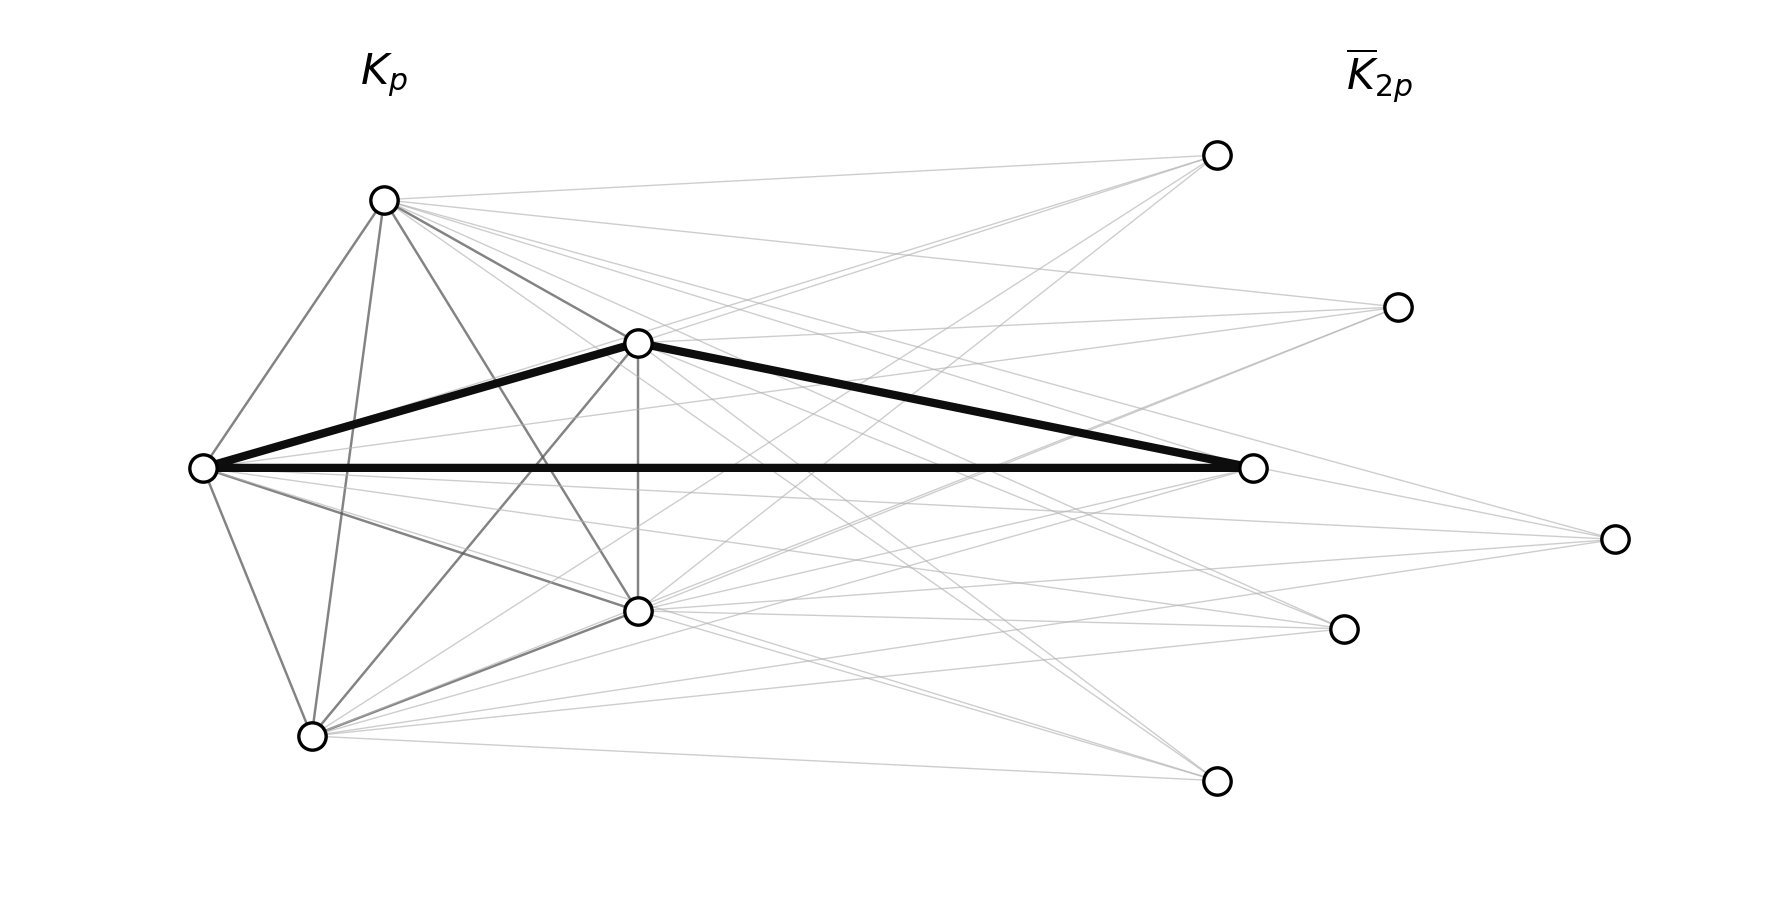
\includegraphics[keepaspectratio,alt={El extremizador complete-split K\_p\textbackslash vee\textbackslash overline K\_\{2p\}. El dibujo es esquemático: el lado izquierdo representa la clique K\_p, el lado derecho representa un conjunto independiente de orden 2p, y están presentes todas las aristas cruzadas. Se destaca un triángulo para mostrar que todo triángulo contiene una arista de la clique.}]{figures/fig1_complete_split_extremizer_es.png}}
\caption{El extremizador complete-split \(K_p\vee\overline K_{2p}\). El dibujo es esquemático: el lado izquierdo representa la clique \(K_p\), el lado derecho representa un conjunto independiente de orden \(2p\), y están presentes todas las aristas cruzadas. Se destaca un triángulo para mostrar que todo triángulo contiene una arista de la clique.}
\end{figure}

\textbf{Figura 1.} El grafo complete-split \(K_p\vee\overline K_{2p}\). Están presentes todas las aristas entre las dos partes, y el lado independiente no contiene aristas internas. Como todo triángulo contiene una arista de la clique, un empaquetamiento de triángulos arista-disjuntos usa a lo sumo \(\binom p2\) triángulos; véase la Sección 10.2. La figura es ilustrativa y no se usa como premisa de la demostración.

\subsection{1.3 Por qué aparece el corredor mesoscópico}\label{por-quuxe9-aparece-el-corredor-mesoscuxf3pico}

El argumento de localización es contabilidad interna de la demostración por contradicción, no una proposición extremal adicional. Supongamos que no existe una cota con error lineal absoluto y, para cada entero positivo \(k\), elijamos un grafo split \(G_k\) de orden mínimo que satisfaga

\[
|E(G_k)|-2\nu_3(G_k)>\frac{|V(G_k)|^2}{6}+k|V(G_k)|.
\]

Tras pasar a una subsucesión y escribir \(|K_k|=p_k\), \(|I_k|=q_k\), toda sucesión hipotética de este tipo debe satisfacer

\[
\frac{q_k}{p_k}\longrightarrow 2.
\]

Además, si \(q_k=2p_k-s_k\), entonces las estimaciones del régimen bulk y del corredor corto fuerzan

\[
\sqrt{p_k}\ll s_k=o(p_k).
\]

Así, la demostración queda forzada al corredor mesoscópico casi extremal. La dicotomía de dispersión alta/baja de la Sección 9 excluye entonces ese corredor. La Sección 10.3 vuelve a esta localización únicamente para explicar la arquitectura de la demostración ya concluida.

\subsection{1.4 Lo que el teorema no prueba}\label{lo-que-el-teorema-no-prueba}

Sea \(\nu_3^*(G)\) el número fraccional de empaquetamiento de triángulos. La presente demostración \textbf{no} establece

\[
\nu_3^*(G)-\nu_3(G)=O(n)
\tag{1.4}
\]

uniformemente sobre grafos split.

En efecto, escribamos

\[
\Gamma(G)=\nu_3^*(G)-\nu_3(G)
\]

y

\[
S(G)=\frac{n^2}{6}-\bigl(|E(G)|-2\nu_3^*(G)\bigr).
\]

Entonces

\[
|E(G)|-2\nu_3(G)
=
\frac{n^2}{6}-S(G)+2\Gamma(G).
\tag{1.5}
\]

Teorema 1.1 solo requiere

\[
2\Gamma(G)\le S(G)+O(n).
\]

En el régimen bulk, \(S(G)\) es cuadrático y absorbe la pérdida general de integralidad \(o(n^2)\). Por tanto, el problema universal de brecha lineal de integralidad sigue abierto.

\subsection{1.5 Arquitectura de la demostración}\label{arquitectura-de-la-demostraciuxf3n}

Escribamos

\[
|K|=p,
\qquad
|I|=q,
\qquad
\alpha=\frac qp.
\]

La razón \(\alpha=q/p\) determina qué fuente de holgura está disponible. Primero resolvemos \(q\ge2p-1\) mediante factorización promediada directa y podemos entonces suponer \(0\le\alpha<2\). Una sucesión hipotética de contraejemplos tiene una subsucesión en uno de tres regímenes.

\begin{enumerate}
\def\labelenumi{\arabic{enumi}.}
\item
  \textbf{Bulk:} \(\alpha\) permanece alejado tanto de \(0\) como de \(2\). Un LP exacto de perfil común y un argumento de clonación fraccional producen holgura fraccional cuadrática. Haxell--Rödl convierte el empaquetamiento fraccional en uno integral con pérdida solo \(o(n^2)\).
\item
  \textbf{Lado independiente escaso:} \(\alpha\to0\). Cada vértice independiente ancla un matching grande dentro de su vecindario. La clique residual es casi completa. Después de eliminar \(O(p)\) aristas para corregir la divisibilidad, admite una descomposición exacta en triángulos.
\item
  \textbf{Corredor cercano al extremo:} \(\alpha\to2\). Escribamos \(q=2p-s\). La factorización promediada cierra \(s=O(\sqrt p)\). Para \(\sqrt p\ll s=o(p)\), la dispersión alta se paga mediante un término de polarización de factor doble, mientras que la dispersión baja implica cercanía a un centro común y se trata mediante completación de ganancia con centro desplazado.
\end{enumerate}

\textbf{Tabla 1. Los tres regímenes de la demostración.} Los regímenes bulk y sparse conservan su procedencia bibliográfica, mientras que el corredor casi extremal es elemental y efectivo.

{\def\LTcaptype{none} % do not increment counter
\begin{longtable}[]{@{}
  >{\raggedright\arraybackslash}p{(\linewidth - 8\tabcolsep) * \real{0.2000}}
  >{\raggedright\arraybackslash}p{(\linewidth - 8\tabcolsep) * \real{0.2000}}
  >{\raggedright\arraybackslash}p{(\linewidth - 8\tabcolsep) * \real{0.2000}}
  >{\raggedright\arraybackslash}p{(\linewidth - 8\tabcolsep) * \real{0.2000}}
  >{\raggedright\arraybackslash}p{(\linewidth - 8\tabcolsep) * \real{0.2000}}@{}}
\toprule\noalign{}
\begin{minipage}[b]{\linewidth}\raggedright
Régimen
\end{minipage} & \begin{minipage}[b]{\linewidth}\raggedright
Condición sobre \(\alpha=q/p\)
\end{minipage} & \begin{minipage}[b]{\linewidth}\raggedright
Fuente de holgura
\end{minipage} & \begin{minipage}[b]{\linewidth}\raggedright
Ingrediente matemático
\end{minipage} & \begin{minipage}[b]{\linewidth}\raggedright
Secciones
\end{minipage} \\
\midrule\noalign{}
\endhead
\bottomrule\noalign{}
\endlastfoot
Lado independiente sparse & \(\alpha\to 0\) & el residual denso de la clique admite una descomposición exacta en triángulos & Dross + Barber--Kühn--Lo--Osthus & §8 \\
Bulk & \(\alpha\) acotado lejos de \(0\) y \(2\) & margen fraccional cuadrático (LP de perfil común + clonación fraccional) & Haxell--Rödl/Yuster & §3--4, §9.1 \\
Corredor casi extremal & \(\alpha\to 2\), \(q=2p-s\) & factorización promediada, polarización de factor doble y completación de ganancia con centro desplazado & ninguno más allá de fundamentos estándar & §5--7, §9.2--9.3, §10.5 \\
\end{longtable}
}

La división no es cosmética. En el bulk hay suficiente holgura fraccional cuadrática para absorber una pérdida general de redondeo \(o(n^2)\). En los dos extremos esa holgura se desvanece, por lo que la demostración reemplaza el redondeo genérico por construcciones adaptadas a la geometría de la presentación split.

\begin{figure}
\centering
\pandocbounded{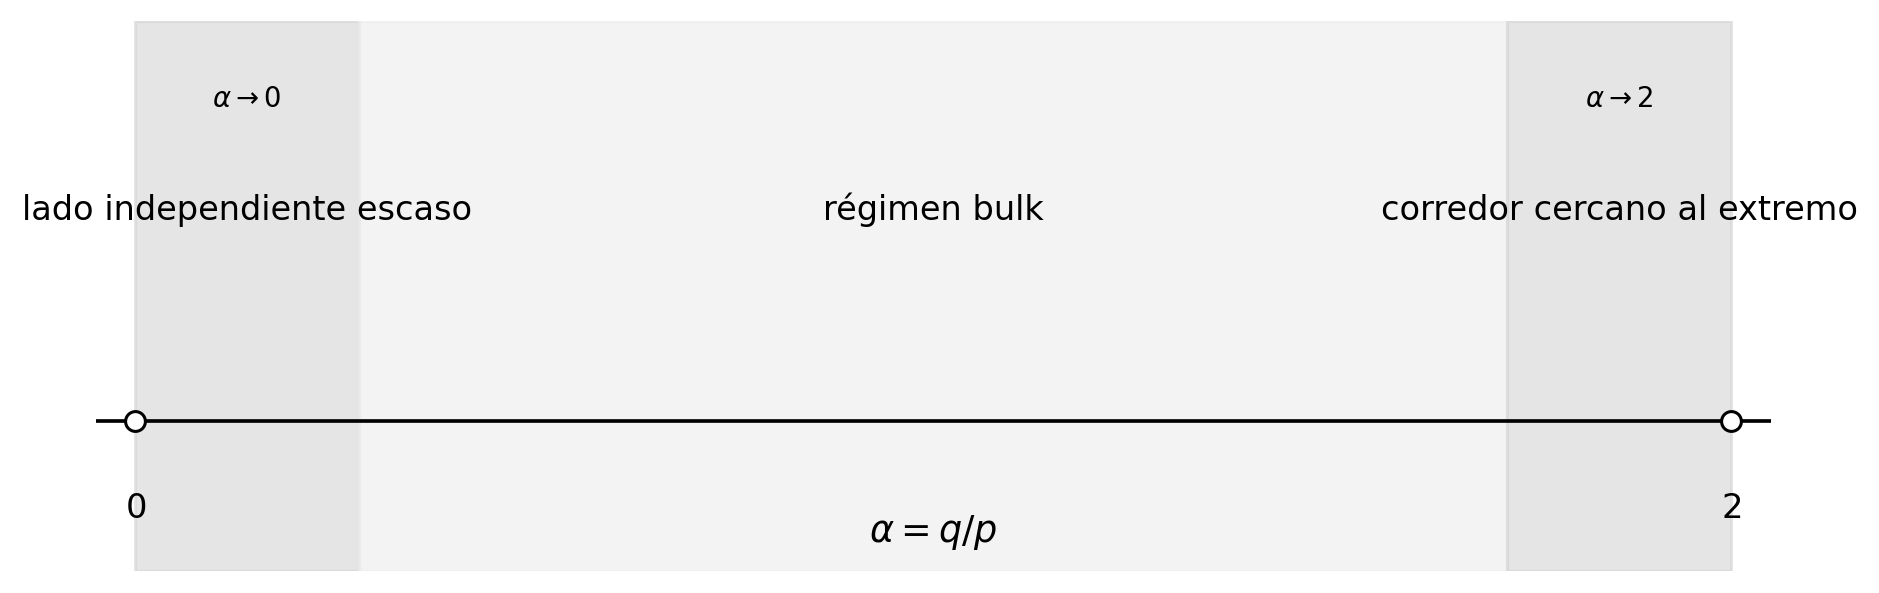
\includegraphics[keepaspectratio,alt={Mapa esquemático de los tres regímenes de la demostración sobre el eje de parámetros \textbackslash alpha=q/p: el régimen escaso cerca de 0, el bulk alejado de ambos extremos y el corredor cercano al extremo cerca de 2.}]{figures/fig2_alpha_regimes_es.png}}
\caption{Mapa esquemático de los tres regímenes de la demostración sobre el eje de parámetros \(\alpha=q/p\): el régimen escaso cerca de \(0\), el bulk alejado de ambos extremos y el corredor cercano al extremo cerca de \(2\).}
\end{figure}

\textbf{Figura 2.} Los tres regímenes de parámetros usados en la demostración. Se muestran los principales umbrales del corredor; las hipótesis completas aparecen en las Secciones 4, 8 y 9. Los regímenes extremos son asintóticos y no subintervalos rígidos de \([0,2]\).

\subsection{1.6 Auditorías computacionales suplementarias}\label{auditoruxedas-computacionales-suplementarias}

El paquete de cierre acompañante contiene pruebas de regresión con aritmética exacta e instancias finitas para identidades seleccionadas y desigualdades cuantitativas usadas en la demostración.

Todo enunciado auditado se prueba analíticamente en el manuscrito. Ningún cálculo, script, enumeración finita ni salida de solver es una premisa lógica de Teorema 1.1. El material suplementario se proporciona únicamente para comprobación independiente, pruebas de regresión y reproducibilidad.

\subsection{1.7 Organización}\label{organizaciuxf3n}

La Sección 2 fija la notación y los teoremas asintóticos usados en la demostración. La Sección 3 resuelve el programa lineal del perfil común. La Sección 4 prueba la cota de clonación fraccional y el margen fraccional global. La Sección 5 desarrolla el redondeo por factorización promediada y doble. La Sección 6 prueba la polarización. La Sección 7 demuestra la desigualdad de centro desplazado. Las Secciones 8--9 cierran los tres regímenes. La Sección 10 reúne las consecuencias cuantitativas y el benchmark afilado. Las Secciones 11--13 registran alcance, problemas abiertos y estado de verificación. Los apéndices contienen los cálculos auxiliares, la demostración autocontenida del coloreo por listas y una selección curada de corolarios formalizados.

\begin{center}\rule{0.5\linewidth}{0.5pt}\end{center}

\section{2. Preliminares}\label{preliminares}

\subsection{2.1 Notación split}\label{notaciuxf3n-split}

En todo el artículo,

\[
G=(K\sqcup I,E)
\]

es un grafo split, donde \(K\) es una clique de tamaño \(p\) e \(I=\{v_1,\ldots,v_q\}\) es independiente.

Para \(v_i\in I\), escribimos

\[
N_i=N(v_i)\cap K,
\qquad
d_i=|N_i|,
\qquad
S_i=K\setminus N_i,
\qquad
m_i=|S_i|.
\]

Definamos

\[
M=\sum_i m_i,
\qquad
S_2=\sum_i m_i^2.
\]

Cuando \(q\) es cercano a \(2p\), escribimos

\[
q=2p-s.
\tag{2.1}
\]

\subsection{2.2 Empaquetamientos de triángulos}\label{empaquetamientos-de-triuxe1ngulos}

Un empaquetamiento fraccional de triángulos es una asignación de pesos no negativos a los triángulos de \(G\) tal que el peso total que pasa por cada arista es a lo sumo uno. Su valor máximo es \(\nu_3^*(G)\).

El dual es una cobertura fraccional de triángulos: una asignación de pesos no negativos a las aristas tal que cada triángulo recibe peso total de aristas al menos uno. La dualidad de programación lineal da igualdad entre ambos valores óptimos.

En todo el artículo escribimos

\[
\Phi(G):=|E(G)|-2\nu_3(G)
\]

para el defecto integral de empaquetamiento de triángulos; por (1.1), \(\operatorname{cp}(G)\le\Phi(G)\).

\subsection{2.3 Factorizaciones de grafos completos}\label{factorizaciones-de-grafos-completos}

Adoptamos las convenciones de frontera

\[
\chi'(K_0)=\chi'(K_1)=0.
\]

Para \(t\ge2\), el índice cromático de un grafo completo es

\[
\chi'(K_t)
=
\begin{cases}
t-1,&t\text{ par},\\
t,&t\text{ impar}.
\end{cases}
\tag{2.2}
\]

Por tanto, \(E(K_t)\) se descompone en \(\chi'(K_t)\) matchings. Las convenciones para \(t\le1\) hacen que el mismo lenguaje sea válido para conjuntos de aristas vacíos.

\subsection{2.4 Teoremas asintóticos usados en la demostración}\label{teoremas-asintuxf3ticos-usados-en-la-demostraciuxf3n}

La demostración escrita usa dos teoremas asintóticos de la literatura. Sus contrapartes formales y su estado de verificación se registran en la Sección 11.6. El caso de coloreo de aristas por listas que aquí se necesita se prueba de forma autocontenida en el Apéndice D. Por tanto, las Secciones 5--7 y la Proposición 10.5 no utilizan insumos asintóticos, aunque emplean hechos estándar como el coloreo de aristas de los grafos completos.

\subsubsection{Teorema 2.1 --- Haxell--Rödl/Yuster {[}11,17{]}}\label{teorema-2.1-haxellruxf6dlyuster-1117}

Para todo grafo fijo \(H\),

\[
\nu_H^*(G)-\nu_H(G)=o(|V(G)|^2)
\]

uniformemente sobre grafos \(G\). Lo aplicamos con \(H=K_3\).

\subsubsection{Teorema 2.2 --- Coloreo de aristas por listas (probado en el Apéndice D)}\label{teorema-2.2-coloreo-de-aristas-por-listas-probado-en-el-apuxe9ndice-d}

Sea \(B\) un grafo bipartito simple de grado máximo \(\Delta(B)\). Si a cada arista \(e\) se le asigna una lista \(L(e)\) con

\[
|L(e)|\ge\Delta(B),
\]

entonces \(B\) tiene un coloreo propio de aristas que elige el color de cada arista desde su lista.

Este es el caso de grado máximo del teorema de Galvin {[}10{]}. En el Apéndice D se da una demostración autocontenida (coloreo de König, emparejamientos estables y el lema del kernel), de modo que no constituye una dependencia externa del artículo. El refinamiento local \(|L(xy)|\ge\max\{d(x),d(y)\}\) de Borodin, Kostochka y Woodall {[}4{]} no es necesario: la hipótesis (7.2) ya acota cada lista por el grado máximo del grafo de ganancia.

\subsubsection{Teorema 2.3 --- Descomposición densa en triángulos}\label{teorema-2.3-descomposiciuxf3n-densa-en-triuxe1ngulos}

Para todo \(\varepsilon>0\), todo grafo \(H\) suficientemente grande, divisible en triángulos y con

\[
\delta(H)\ge(0.9+\varepsilon)|V(H)|
\]

admite una descomposición en triángulos. Esto se sigue del teorema de descomposición fraccional en triángulos de Dross {[}7{]} (grado mínimo \(0.9v\) basta fraccionalmente), combinado con el teorema de absorción iterativa de Barber, Kühn, Lo y Osthus {[}2{]}, que convierte el umbral fraccional en un umbral de descomposición exacta para grafos divisibles en triángulos, salvo \(\varepsilon\) y para orden suficientemente grande.

\paragraph{\texorpdfstring{Observación 2.3\(^{\prime}\) --- Necesidad de una hipótesis de densidad}{Observación 2.3\^{}\{\textbackslash prime\} --- Necesidad de una hipótesis de densidad}}\label{observaciuxf3n-2.3prime-necesidad-de-una-hipuxf3tesis-de-densidad}

La divisibilidad por triángulos no implica por sí sola descomponibilidad en triángulos. El ciclo de longitud seis tiene todos sus grados pares y un número de aristas divisible por \(3\), pero no admite una descomposición en triángulos. Una segunda obstrucción se obtiene de \(K_7\) eliminando dos triángulos disjuntos en vértices: el grafo resultante es divisible por triángulos y tiene \(15\) aristas, pero tampoco se descompone en triángulos. Por tanto, un teorema de descomposición para grafos divisibles por triángulos requiere una hipótesis adicional, como la condición de densidad del Teorema 2.3. Estos ejemplos motivan esa hipótesis; no son premisas del Teorema 2.3 ni del Teorema 1.1.

\textbf{Certificados Lean.} \texttt{PaperIII.ax2\_divisibility\_degree\_insufficient}, \texttt{PaperIII.ax2\_density\_necessary\_K7\_minus\_two\_triangles}, reexportados mediante \texttt{PaperIII.Obstructions}.

\subsection{2.5 Interfaces auxiliares formalizadas}\label{interfaces-auxiliares-formalizadas}

El desarrollo formal registra consecuencias que van más allá de la demostración principal. El Apéndice E conserva solo aquellas que afinan las construcciones centrales del artículo o son reutilizables fuera de la aplicación a grafos split: cotas de empaquetamiento por factorización, estimaciones seleccionadas del corredor, el valor exacto del perfil común, el margen fraccional unificado, el paquete de sharpness complete-split, dualidad LP finita, limpieza mediante matchings y una interfaz de nibble \(r\)-uniforme. Las ventanas de grados al nivel de implementación, los lemas de codificación de hipergrafos tipados, los wrappers de monotonía y las formas numéricas duplicadas permanecen disponibles en las fuentes Lean, pero no se repiten en el manuscrito.

Estas interfaces son consecuencias o infraestructura de demostración, no premisas adicionales del Teorema 1.1. Su estado de release se registra en las Secciones 11.6 y 13.

\begin{center}\rule{0.5\linewidth}{0.5pt}\end{center}

\section{3. El programa lineal de perfil común}\label{el-programa-lineal-de-perfil-comuxfan}

Para enteros \(p,q,d\), sea \(H(p,q,d)\) el grafo split con clique \(K\), \(|K|=p\), conjunto independiente \(I\), \(|I|=q\), y un conjunto fijo \(N\subseteq K\), \(|N|=d\), tal que todo vértice de \(I\) tiene vecindario \(N\). Definamos \(R=K\setminus N\) y \(r=p-d\).

\subsection{3.1 Variables simétricas de cobertura}\label{variables-simuxe9tricas-de-cobertura}

Al promediar sobre permutaciones de \(N\), \(R\) e \(I\), puede suponerse que una cobertura fraccional óptima de triángulos es constante sobre las cuatro clases de aristas

\[
E(N),
\qquad E(N,I),
\qquad E(N,R),
\qquad E(R).
\]

Sean \(a,b,c,e\) sus pesos respectivos. Las restricciones de triángulos son

\[
a+2b\ge1,
\qquad
3a\ge1,
\tag{3.1}
\]

\[
a+2c\ge1,
\qquad
2c+e\ge1,
\qquad
3e\ge1.
\tag{3.2}
\]

Las restricciones correspondientes a tipos de triángulos vacíos pueden omitirse; la fórmula siguiente sigue siendo válida para \(p\ge3\).

El objetivo es

\[
\binom d2a+qdb+dr\,c+\binom r2e.
\tag{3.3}
\]

\subsection{3.2 Solución exacta}\label{soluciuxf3n-exacta}

\subsubsection{Teorema 3.1 --- Fórmula de perfil común}\label{teorema-3.1-fuxf3rmula-de-perfil-comuxfan}

Para \(p\ge3\) y \(q\ge1\),

\[
\boxed{
\nu_3^*(H(p,q,d))
=
F(p,q,d),
}
\tag{3.4}
\]

donde

\[
\boxed{
F(p,q,d)
=
\min\left\{
\frac{\binom p2+qd}{3},
\binom d2+\binom r2,
\binom d2+\frac{dr+\binom r2}{3}
\right\}.
}
\tag{3.5}
\]

\subsubsection{Demostración}\label{demostraciuxf3n}

En un óptimo,

\[
b=\frac{1-a}{2},
\qquad
c=\frac{1-\min\{a,e\}}2,
\qquad
\frac13\le a,e\le1.
\]

Si \(a\le e\), disminuir \(e\) hasta \(a\) no puede aumentar el objetivo. Por tanto, basta minimizar sobre

\[
\frac13\le e\le a\le1.
\]

El objetivo es afín sobre este triángulo, por lo que un mínimo ocurre en

\[
(a,e)=\left(\frac13,\frac13\right),
\qquad
(1,1),
\qquad
\left(1,\frac13\right).
\]

Los valores correspondientes son precisamente las tres expresiones de (3.5). La dualidad completa la demostración. \(\square\)

Cuando \(q=0\), el grafo \(H(p,0,d)\) es simplemente \(K_p\), independientemente de \(d\), y la misma fórmula se sigue de \(\nu_3^*(K_p)=\binom p2/3\).

\subsection{3.3 Interpretación de las tres coberturas}\label{interpretaciuxf3n-de-las-tres-coberturas}

El mínimo de (3.5) se recuerda con mayor facilidad mediante los tres vértices del programa reducido de dos variables. Cada vértice representa una manera distinta de pagar las restricciones de triángulos.

{\def\LTcaptype{none} % do not increment counter
\begin{longtable}[]{@{}
  >{\raggedright\arraybackslash}p{(\linewidth - 6\tabcolsep) * \real{0.2143}}
  >{\raggedleft\arraybackslash}p{(\linewidth - 6\tabcolsep) * \real{0.2857}}
  >{\raggedleft\arraybackslash}p{(\linewidth - 6\tabcolsep) * \real{0.2857}}
  >{\raggedright\arraybackslash}p{(\linewidth - 6\tabcolsep) * \real{0.2143}}@{}}
\toprule\noalign{}
\begin{minipage}[b]{\linewidth}\raggedright
Patrón de cobertura
\end{minipage} & \begin{minipage}[b]{\linewidth}\raggedleft
Vértice reducido \((a,e)\)
\end{minipage} & \begin{minipage}[b]{\linewidth}\raggedleft
Valor
\end{minipage} & \begin{minipage}[b]{\linewidth}\raggedright
Descripción geométrica
\end{minipage} \\
\midrule\noalign{}
\endhead
\bottomrule\noalign{}
\endlastfoot
\textbf{Uniforme} & \((1/3,1/3)\) & \(\bigl(\binom p2+qd\bigr)/3\) & Todas las órbitas relevantes de aristas se cubren a la tasa fraccional uniforme. \\
\textbf{Separada} & \((1,1)\) & \(\binom d2+\binom r2\) & Los dos bloques de clique \(N\) y \(R\) se pagan internamente, sin peso sobre la órbita cruzada. \\
\textbf{Vecindario caliente} & \((1,1/3)\) & \(\binom d2+\bigl(dr+\binom r2\bigr)/3\) & El vecindario común \(N\) se paga por completo, mientras la estructura de clique residual permanece fraccional. \\
\end{longtable}
}

Las etiquetas son descriptivas y no constituyen definiciones adicionales. En los cálculos posteriores nos referimos a las correspondientes ramas primera, segunda y tercera de \(F\). Esta tricotomía finita es la fuente del margen fraccional global.

\begin{center}\rule{0.5\linewidth}{0.5pt}\end{center}

\section{4. Clonación fraccional y margen fraccional exacto}\label{clonaciuxf3n-fraccional-y-margen-fraccional-exacto}

\subsection{4.1 Clonación fraccional}\label{clonaciuxf3n-fraccional}

La operación de clonación fraccional (replicación) usada aquí es el análogo, desde el lado de coberturas, de la simetrización por clones usada en Paper II. Allí, vértices o clases de clones se copian por pares para simplificar un grafo cordal. Aquí, un perfil del conjunto independiente se copia \(q\) veces en un solo paso de promediado; el grafo \(H(p,q,d_i)\) registra el perfil común resultante.

\subsubsection{Lema 4.1 --- Cota de clonación fraccional}\label{lema-4.1-cota-de-clonaciuxf3n-fraccional}

Para todo grafo split con \(q\ge1\),

\[
\boxed{
\nu_3^*(G)
\ge
\frac1q\sum_{i=1}^qF(p,q,d_i).
}
\tag{4.1}
\]

\subsubsection{Demostración}\label{demostraciuxf3n-1}

Sea \(y\) una cobertura fraccional cualquiera de triángulos de \(G\). Definamos

\[
A=\sum_{e\in E(K)}y_e
\]

y

\[
B_i=\sum_{x\in N_i}y_{v_ix}.
\]

Reemplacemos \(v_i\) por \(q\) clones independientes, todos con vecindario \(N_i\), y demos a cada clone los pesos incidentes de \(v_i\). Junto con los pesos originales de las aristas de la clique, esto es una cobertura fraccional de \(H(p,q,d_i)\) de peso \(A+qB_i\). Por tanto,

\[
A+qB_i\ge F(p,q,d_i).
\]

Al sumar sobre \(i\) obtenemos

\[
q\left(A+\sum_iB_i\right)
\ge
\sum_iF(p,q,d_i).
\]

Minimizar sobre las coberturas prueba el lema. \(\square\)

\subsection{4.2 El margen exacto}\label{el-margen-exacto}

Supongamos \(0<q\le2p\), definamos

\[
\alpha=\frac qp,
\]

y el umbral de empaquetamiento

\[
T(G)=\frac12\left(|E(G)|-\frac{(p+q)^2}{6}\right).
\tag{4.2}
\]

Definamos

\[
\mu(\alpha)
=
\begin{cases}
\alpha^2/12,&0\le\alpha\le2/3,\\
(2-\alpha)^2/48,&2/3\le\alpha\le2.
\end{cases}
\tag{4.3}
\]

\subsubsection{Teorema 4.2 --- Margen fraccional unificado}\label{teorema-4.2-margen-fraccional-unificado}

\[
\boxed{
\nu_3^*(G)
\ge
T(G)+\mu(\alpha)p^2-\frac p4.
}
\tag{4.4}
\]

\subsubsection{Demostración}\label{demostraciuxf3n-2}

Sea

\[
C_\alpha=\frac{2-2\alpha-\alpha^2}{12}.
\]

Para cada rama de \(F(p,q,d)\), completar cuadrados da

\[
F(p,q,d)
\ge
\frac{qd}{2}+C_\alpha p^2+\mu(\alpha)p^2-\frac p2.
\tag{4.5}
\]

Los tres mínimos residuales normalizados son

\[
\frac{\alpha^2}{12},
\qquad
\frac{(2-\alpha)^2}{48},
\]

y

\[
\begin{cases}
\alpha(8-5\alpha)/48,&\alpha\le4/3,\\
(2-\alpha)^2/12,&\alpha\ge4/3.
\end{cases}
\]

El tercero nunca está por debajo del mínimo de los dos primeros. Promediar (4.5) mediante Lema 4.1 da

\[
\nu_3^*(G)
\ge
\frac12\sum_i d_i+C_\alpha p^2+\mu(\alpha)p^2-\frac p2.
\]

Como

\[
T(G)=\frac12\sum_i d_i+C_\alpha p^2-\frac p4,
\]

obtenemos (4.4). \(\square\)

\subsection{4.3 Consecuencia para el bulk}\label{consecuencia-para-el-bulk}

Si

\[
\varepsilon\le\alpha\le2-\varepsilon,
\]

entonces \(\mu(\alpha)\ge c_\varepsilon>0\). Teorema 4.2 y Haxell--Rödl implican

\[
\nu_3(G)\ge T(G)
\]

para todos los grafos suficientemente grandes en este régimen. Por tanto,

\[
|E(G)|-2\nu_3(G)
\le
\frac{n^2}{6}.
\tag{4.6}
\]

\begin{center}\rule{0.5\linewidth}{0.5pt}\end{center}

\section{\texorpdfstring{5. Redondeo por factorización cerca de \(q=2p\)}{5. Redondeo por factorización cerca de q=2p}}\label{redondeo-por-factorizaciuxf3n-cerca-de-q2p}

Sea

\[
r_p=\chi'(K_p).
\]

\subsection{5.1 Promediado con un factor}\label{promediado-con-un-factor}

\subsubsection{Lema 5.1}\label{lema-5.1}

Si \(q\ge r_p\), entonces

\[
\boxed{
\nu_3(G)
\ge
\frac1q\sum_i\binom{d_i}{2}.
}
\tag{5.1}
\]

\subsubsection{Demostración}\label{demostraciuxf3n-3}

Factorizamos \(K_p\) en \(r_p\) matchings. Asignamos los factores de manera inyectiva y uniforme a vértices de \(I\). En el factor asignado a \(v_i\), conservamos solo las aristas cuyos dos extremos pertenecen a \(N_i\). Las aristas conservadas forman triángulos \(KKI\) válidos y arista-disjuntos.

El número esperado de aristas conservadas es

\[
\frac1q\sum_i\sum_{j=1}^{r_p}|F_j\cap E(K[N_i])|
=
\frac1q\sum_i\binom{d_i}{2}.
\]

Alguna asignación alcanza al menos la esperanza. \(\square\)

El Apéndice E.1 registra la desigualdad de empaquetamiento al nivel de asignaciones, antes de promediar, junto con su certificado Lean.

Al escribir \(q=2p-s\), la sustitución da

\[
\Phi(G)
\le
\frac{n^2}{6}+\frac p2-\frac{s^2}{6}
+
\frac{(s-1)M-S_2}{q}.
\tag{5.2}
\]

Usando \(S_2\ge M^2/q\) y maximizando la parábola resultante se obtiene

\[
\boxed{
\Phi(G)
\le
\frac{n^2}{6}+\frac p2+\frac{s^2-6s+3}{12}.
}
\tag{5.3}
\]

Así, \(s=O(\sqrt p)\) queda cerrado con error lineal.

\subsection{5.2 Redondeo con factor doble}\label{redondeo-con-factor-doble}

Para una arista \(e=xy\) de la clique, sea

\[
b_e=|\{i:\{x,y\}\not\subseteq N_i\}|.
\]

Definamos

\[
h=\min\{r_p,q-r_p\},
\qquad
\delta=\frac h{r_p}.
\]

Elegimos uniformemente al azar el conjunto de \(h\) factores que reciben dos vértices independientes distintos, damos un vértice independiente a cada factor restante y asignamos los vértices independientes a las posiciones resultantes de manera uniforme e inyectiva. Todas las esperanzas siguientes se toman respecto de ambas elecciones aleatorias; alguna elección determinista alcanza al menos la ganancia esperada.

\subsubsection{Lema 5.2 --- Desigualdad de factor doble}\label{lema-5.2-desigualdad-de-factor-doble}

Si \(q\ge r_p\), entonces

\[
\boxed{
\begin{aligned}
\Phi(G)
\le{}&
\frac{n^2}{6}+\frac p2-\frac{s^2}{6}
+
\frac{(s-1)M-S_2}{q}\\
&-
\frac{2\delta V}{q(q-1)},
\end{aligned}
}
\tag{5.4}
\]

donde

\[
V=\sum_{e\in E(K)}b_e(q-b_e).
\tag{5.5}
\]

\subsubsection{Demostración}\label{demostraciuxf3n-4}

Si el factor que contiene a \(e\) recibe un vértice, \(e\) se pierde con probabilidad \(b_e/q\). Si recibe dos vértices, se pierde solo cuando ambos son malos, con probabilidad

\[
\frac{b_e(b_e-1)}{q(q-1)}.
\]

Por tanto, el número esperado \(U\) de aristas de clique perdidas es

\[
U
=
\frac1q\sum_e b_e
-
\frac{\delta}{q(q-1)}\sum_e b_e(q-b_e).
\]

Como cada factor es un matching, cada arista conservada puede asignarse a uno de sus vértices admisibles sin crear una colisión de aristas. La sustitución da (5.4). \(\square\)

La cota inferior correspondiente, formulada directamente en términos de empaquetamientos, aparece como Corolario E.1.2.

\begin{center}\rule{0.5\linewidth}{0.5pt}\end{center}

\section{6. Polarización cuantitativa}\label{polarizaciuxf3n-cuantitativa}

Para cada \(i\), definamos

\[
\mathcal B_i=\{e\in E(K):e\cap S_i\ne\varnothing\}.
\]

Entonces

\[
V=\sum_{i,j}|\mathcal B_i\setminus\mathcal B_j|.
\tag{6.1}
\]

Sea

\[
m=\max_i|S_i|.
\]

\subsubsection{Lema 6.1 --- Desigualdad de polarización}\label{lema-6.1-desigualdad-de-polarizaciuxf3n}

Si \(2p-3m-1\ge0\), entonces

\[
\boxed{
V
\ge
\frac{2p-3m-1}{4}
\sum_{i,j}|S_i\triangle S_j|.
}
\tag{6.2}
\]

\subsubsection{Demostración}\label{demostraciuxf3n-5}

Definamos

\[
a_{ij}=|S_i\setminus S_j|.
\]

Las aristas de \(\mathcal B_i\setminus\mathcal B_j\) son precisamente las aristas de \(K_p-S_j\) que inciden en \(S_i\setminus S_j\). Por tanto,

\[
|\mathcal B_i\setminus\mathcal B_j|
=
\frac{a_{ij}\bigl(2(p-|S_j|)-a_{ij}-1\bigr)}2.
\]

Como \(|S_j|\le m\) y \(a_{ij}\le m\),

\[
|\mathcal B_i\setminus\mathcal B_j|
\ge
\frac{2p-3m-1}{2}|S_i\setminus S_j|.
\]

Sumamos sobre pares ordenados y usamos

\[
\sum_{i,j}|S_i\setminus S_j|
=
\frac12\sum_{i,j}|S_i\triangle S_j|.
\]

Esto prueba (6.2). \(\square\)

\begin{center}\rule{0.5\linewidth}{0.5pt}\end{center}

\section{7. Completación de ganancia con centro desplazado}\label{completaciuxf3n-de-ganancia-con-centro-desplazado}

Fijemos \(R\subseteq K\). Definamos

\[
\rho=|R|,
\qquad
Q=K\setminus R,
\qquad
b=|Q|.
\]

Para cada \(i\), definamos

\[
T_i=S_i\setminus R,
\qquad
t_i=|T_i|,
\]

y

\[
G_i=R\setminus S_i,
\qquad
g_i=|G_i|.
\]

Definamos

\[
A_R=\sum_i t_i,
\qquad
A_{2,R}=\sum_i t_i^2,
\qquad
B_R=\sum_i g_i.
\]

Sea

\[
r_b=\chi'(K_b),
\qquad
u=q-r_b.
\]

Supongamos

\[
b\ge2,
\qquad
q\ge r_b,
\qquad
b\ge\chi'(K_\rho),
\tag{7.1}
\]

y

\[
b-t_i\ge\max\{\rho,u\}
\qquad
\text{para todo }i.
\tag{7.2}
\]

Definamos

\[
\theta_R=\frac{\max\{\rho-1,0\}}{b}
\]

y

\[
\kappa_R
=
1-2(1-\theta_R)\frac{u}{q}.
\tag{7.3}
\]

\subsection{\texorpdfstring{7.1 Empaquetamiento dentro de \(Q\)}{7.1 Empaquetamiento dentro de Q}}\label{empaquetamiento-dentro-de-q}

Reservamos un conjunto \(U\subseteq I\) de \(u\) vértices; nótese que \(|I\setminus U|=q-u=r_b\) exactamente. Asignamos los \(r_b\) vértices restantes biyectivamente a una factorización de \(K[Q]\).

Para \(v_i\), el número de aristas no disponibles de \(K[Q]\) es

\[
\beta_i
=
\binom b2-\binom{b-t_i}{2}.
\tag{7.4}
\]

Para \(U\) fijo, el promediado sobre las asignaciones da al menos

\[
\binom b2-\frac1{r_b}\sum_{i\notin U}\beta_i
\tag{7.5}
\]

triángulos \(QQI\) arista-disjuntos.

\subsection{7.2 El grafo de ganancia}\label{el-grafo-de-ganancia}

Construimos un grafo bipartito con partes \(U\) y \(R\), uniendo \(v_i\) con \(r\) cuando \(r\in G_i\). Asignamos la lista

\[
L(v_ir)=N_i\cap Q.
\]

Por (7.2), toda lista satisface

\[
|L(v_ir)|=b-t_i
\ge
\max\{\rho,u\}
\ge
\Delta,
\]

donde \(\Delta\) es el grado máximo del grafo de ganancia, pues \(d(v_i)=g_i\le\rho\) y \(d(r)\le|U|=u\). Teorema 2.2, probado de manera autocontenida en el Apéndice D, da un coloreo propio de aristas por listas. Si \(v_ir\) recibe el color \(z\in Q\), tomamos el triángulo \(v_irz\). Esto produce

\[
B_U=\sum_{i\in U}g_i
\]

triángulos \(IRQ\) arista-disjuntos.

\subsection{\texorpdfstring{7.3 Completación dentro de \(R\)}{7.3 Completación dentro de R}}\label{completaciuxf3n-dentro-de-r}

Para cada \(z\in Q\), sea \(U_z\subseteq R\) el conjunto de vértices \(r\) para los cuales la arista \(rz\) fue usada por un triángulo \(IRQ\).

Si \(\rho\le1\), el grafo \(K[R]\) no tiene aristas, de modo que esta completación no aporta triángulos \(RRQ\). Supongamos entonces \(\rho\ge2\). Factorizamos \(K[R]\), inyectamos sus factores en los colores \(z\in Q\) y eliminamos del factor asignado a \(z\) toda arista incidente en \(U_z\). El promediado sobre las inyecciones pierde a lo sumo

\[
\frac{\rho-1}{b}\sum_z|U_z|
=
\theta_RB_U
\]

aristas. Por tanto, en todos los casos obtenemos al menos

\[
\binom\rho2-\theta_RB_U
\]

triángulos \(RRQ\) adicionales.

Las tres familias \(QQI\), \(IRQ\) y \(RRQ\) son arista-disjuntas. En particular, la eliminación de colores prohibidos impide que un triángulo \(IRQ\) y un triángulo \(RRQ\) compartan una arista \(rz\).

\subsection{7.4 La desigualdad centrada}\label{la-desigualdad-centrada}

Elegimos \(U\), \(|U|=u\), que maximice

\[
\sum_{i\in U}
\left(
\frac{2\beta_i}{r_b}+2(1-\theta_R)g_i
\right).
\]

Los mejores \(u\) términos tienen suma al menos \(u/q\) veces la suma total. Usando

\[
2\sum_i\beta_i
=(2b-1)A_R-A_{2,R},
\]

obtenemos el lema local principal. La forma de empaquetamiento sobre un host restringido se registra como Corolario E.1.3.

\subsubsection{Lema 7.1 --- Desigualdad con centro desplazado y ganancia reservada}\label{lema-7.1-desigualdad-con-centro-desplazado-y-ganancia-reservada}

Bajo (7.1)--(7.2),

\[
\boxed{
\begin{aligned}
\Phi(G)
\le{}&
\frac{n^2}{6}+\frac p2-\frac{s^2}{6}
+s\rho-2\rho^2\\
&+
\kappa_RB_R
+
\frac{(s-2\rho-1)A_R-A_{2,R}}q.
\end{aligned}
}
\tag{7.6}
\]

\begin{center}\rule{0.5\linewidth}{0.5pt}\end{center}

\section{8. El régimen con lado independiente escaso}\label{el-ruxe9gimen-con-lado-independiente-escaso}

Supongamos \(q=o(p)\). Probamos la cota requerida de forma directa e integral.

\subsection{8.1 Cota de grado en un contraejemplo mínimo}\label{cota-de-grado-en-un-contraejemplo-muxednimo}

En el argumento global por contradicción, un contraejemplo mínimo con penalización \(kn\) satisface, para todo \(v\in I\),

\[
d(v)>
\frac{2n-1}{6}+k.
\tag{8.1}
\]

Como \(q=o(p)\), esto implica eventualmente

\[
d(v)\ge2q+2.
\tag{8.2}
\]

\subsection{8.2 Matchings sucesivos}\label{matchings-sucesivos}

Ordenamos \(I=\{v_1,\ldots,v_q\}\). Elegimos sucesivamente matchings arista-disjuntos

\[
M_i\subseteq K[N_i]
\]

de tamaño \(\lfloor d_i/2\rfloor\).

Antes de elegir \(M_i\), cada vértice ha perdido a lo sumo \(i-1\) aristas incidentes, por lo que el grafo disponible sobre \(N_i\) tiene grado mínimo al menos

\[
d_i-i\ge d_i/2.
\]

El teorema de Dirac {[}6{]} proporciona un ciclo hamiltoniano y, por tanto, un matching del tamaño requerido.

Sea

\[
F=\bigcup_iM_i.
\]

Entonces

\[
|F|
\ge
\frac12\sum_i d_i-\frac q2,
\qquad
\Delta(F)\le q.
\tag{8.3}
\]

Las aristas de \(M_i\) producen \(|M_i|\) triángulos \(KKI\) arista-disjuntos con ápice \(v_i\).

\subsection{8.3 Corrección de divisibilidad}\label{correcciuxf3n-de-divisibilidad}

El grafo residual de la clique

\[
R_0=K_p-F
\]

satisface

\[
\delta(R_0)
\ge
p-1-q
=(1-o(1))p.
\tag{8.4}
\]

En particular, para todos los miembros suficientemente grandes de la sucesión, \(\delta(R_0)>p/2\). El teorema de Dirac {[}6{]} da entonces un ciclo hamiltoniano y, por tanto, un camino hamiltoniano

\[
P=x_1x_2\cdots x_p
\]

contenido en \(R_0\). Sea \(O\) el conjunto de vértices de grado impar de \(R_0\). Por el lema del apretón de manos, \(|O|\) es par. Definimos el subgrafo de camino \(J\subseteq P\) mediante

\[
x_jx_{j+1}\in E(J)
\quad\Longleftrightarrow\quad
|O\cap\{x_1,\ldots,x_j\}|\text{ es impar}.
\tag{8.5}
\]

Para un vértice interno \(x_j\), la paridad de su grado en \(J\) es el cambio de paridad del prefijo entre las posiciones \(j-1\) y \(j\), y por tanto es \(1\) precisamente cuando \(x_j\in O\). La misma conclusión vale en los dos extremos porque \(|O|\) es par. En consecuencia,

\[
\operatorname{Odd}(J)=O,
\qquad
|E(J)|\le p-1,
\qquad
\Delta(J)\le2.
\tag{8.6}
\]

Así,

\[
R_1:=R_0-J
\]

tiene todos sus grados pares, y

\[
\delta(R_1)\ge p-1-q-2.
\tag{8.7}
\]

Como \(q=o(p)\), eventualmente \(\delta(R_1)>3p/4\). Por el teorema de Turán, \(R_1\) contiene una copia de \(K_5\). Elegimos un \(C_4\) y un \(C_5\) dentro de este \(K_5\) fijo. Según

\[
|E(R_1)|\equiv0,1,2\pmod3,
\]

eliminamos respectivamente nada, el \(C_4\) o el \(C_5\). Sea \(C\) el ciclo eliminado, permitiendo \(C=\varnothing\), y definamos

\[
H:=R_1-E(C).
\]

Cada vértice pierde cero o dos aristas incidentes al eliminar un ciclo, de modo que todos los grados de \(H\) siguen siendo pares. Además, \(|E(C)|\equiv |E(R_1)|\pmod3\), y por ello

\[
|E(H)|\equiv0\pmod3.
\]

Por tanto, \(H\) es divisible en triángulos. La pérdida total de grado al pasar de \(R_0\) a \(H\) es a lo sumo cuatro, por lo que

\[
\delta(H)\ge p-1-q-4.
\tag{8.8}
\]

Para aplicar Teorema 2.3 con un parámetro fijo, tomemos por ejemplo \(\varepsilon_0=1/100\). Como \(q=o(p)\), eventualmente \(q\le p/20\), y entonces, para \(p\) suficientemente grande,

\[
\delta(H)\ge p-1-q-4\ge0.91p=(0.9+\varepsilon_0)|V(H)|.
\tag{8.9}
\]

Teorema 2.3 da ahora una descomposición exacta en triángulos de \(H\). Nótese que el teorema de descomposición se aplica sobre el conjunto original de \(p\) vértices: no se elimina ningún vértice durante la corrección. La corrección completa elimina a lo sumo \(p+4\) aristas.

\subsection{8.4 Tamaño del empaquetamiento}\label{tamauxf1o-del-empaquetamiento}

El empaquetamiento combinado tiene tamaño

\[
\begin{aligned}
\nu_3(G)
&\ge
|F|+\frac{\binom p2-|F|-O(p)}3\\
&=
\frac13\binom p2+\frac23|F|-O(p)\\
&\ge
\frac13\binom p2+\frac13\sum_i d_i-O(p+q).
\end{aligned}
\tag{8.10}
\]

En consecuencia,

\[
\begin{aligned}
\Phi(G)
&\le
\frac13\binom p2+\frac13\sum_i d_i+O(p+q)\\
&\le
\frac13\binom p2+\frac{pq}{3}+O(p+q)\\
&=
\frac{(p+q)^2}{6}-\frac{p+q^2}{6}+O(p+q).
\end{aligned}
\tag{8.11}
\]

Esto es a lo sumo \(n^2/6+O(n)\). El Apéndice E.6 registra las interfaces formalizadas de limpieza por matchings y corrección acotada de divisibilidad usadas en este régimen.

\begin{center}\rule{0.5\linewidth}{0.5pt}\end{center}

\section{9. Demostración del teorema principal}\label{demostraciuxf3n-del-teorema-principal}

Probamos ahora Teorema 1.1 por contradicción.

Supongamos que ninguna constante absoluta funciona. Para cada entero positivo \(k\), elegimos un grafo split \(G_k\), mínimo en su número \(n_k\) de vértices, tal que

\[
\Phi(G_k)
>
\frac{n_k^2}{6}+kn_k.
\tag{9.1}
\]

Necesariamente \(n_k\to\infty\). Para todo \(v\in I(G_k)\), la minimalidad da

\[
\Phi(G_k)
\le
\Phi(G_k-v)+d(v),
\]

y por tanto

\[
\boxed{
d(v)>
\frac{2n_k-1}{6}+k.
}
\tag{9.2}
\]

Primero, si \(q_k\ge2p_k-1\), Lema 5.1 da

\[
\Phi(G_k)
\le
\frac{n_k^2}{6}+\frac{p_k}{2},
\]

lo que contradice (9.1) para \(k\) grande. Podemos entonces suponer \(q_k<2p_k-1\) y pasar a una subsucesión de acuerdo con

\[
\alpha_k=\frac{q_k}{p_k}\in[0,2).
\]

\subsection{9.1 Régimen bulk}\label{ruxe9gimen-bulk}

Supongamos que para algún \(\varepsilon>0\),

\[
\varepsilon\le\alpha_k\le2-\varepsilon.
\]

Teorema 4.2 da

\[
\nu_3^*(G_k)
\ge
T(G_k)+c_\varepsilon p_k^2-O(p_k).
\]

Haxell--Rödl da

\[
\nu_3(G_k)
\ge
\nu_3^*(G_k)-o(n_k^2).
\]

Para \(k\) suficientemente grande, el margen cuadrático domina la pérdida de integralidad, por lo que \(\nu_3(G_k)\ge T(G_k)\), en contradicción con (9.1).

\subsection{\texorpdfstring{9.2 El extremo \(\alpha_k\to0\)}{9.2 El extremo \textbackslash alpha\_k\textbackslash to0}}\label{el-extremo-alpha_kto0}

Este caso queda cerrado por la Sección 8, que da una constante absoluta \(C_0\) tal que

\[
\Phi(G_k)
\le
\frac{n_k^2}{6}+C_0n_k.
\]

Para \(k>C_0\), esto contradice (9.1).

\subsection{\texorpdfstring{9.3 El extremo \(\alpha_k\to2\)}{9.3 El extremo \textbackslash alpha\_k\textbackslash to2}}\label{el-extremo-alpha_kto2}

Escribamos

\[
q=2p-s,
\qquad
s=o(p).
\]

Si \(s=O(\sqrt p)\), la desigualdad (5.3) da la cota de error lineal requerida. Supongamos en adelante

\[
\sqrt p\ll s=o(p).
\tag{9.3}
\]

Para todos los miembros suficientemente grandes de la sucesión,

\[
p\ge2304,
\qquad
6\sqrt p\le s\le\frac p8,
\qquad
k\ge1.
\tag{9.4}
\]

Por (9.2),

\[
m_i=|S_i|
<
\frac s3+\frac16-k
\le
\frac s3-\frac56.
\]

Como todo \(m_i\) es entero, con \(m=\max_i m_i\),

\[
\boxed{3m\le s-3.}
\tag{9.5}
\]

Para \(x\in K\), definamos

\[
a_x=|\{i:x\in S_i\}|
\]

y

\[
D=\sum_{x\in K}a_x(q-a_x).
\tag{9.6}
\]

Entonces

\[
\sum_{i,j}|S_i\triangle S_j|=2D.
\tag{9.7}
\]

\subsubsection{Dispersión alta}\label{dispersiuxf3n-alta}

Supongamos

\[
D\ge\frac{qs^2}{12}.
\tag{9.8}
\]

Por (9.5),

\[
2p-3m-1\ge2p-s+2=q+2.
\]

Lema 6.1 y (9.7) dan entonces

\[
V
\ge
\frac{q+2}{2}D
\ge
\frac q2D.
\tag{9.9}
\]

El coeficiente de factor doble de Lema 5.2 satisface

\[
\boxed{\delta\ge\frac78.}
\tag{9.10}
\]

En efecto, si \(p\) es impar, \(r_p=p\) y

\[
\delta=\frac{p-s}{p}\ge\frac78,
\]

mientras que si \(p\) es par, \(r_p=p-1\) y

\[
\delta=\frac{p+1-s}{p-1}\ge\frac78.
\]

Además, \(S_2\ge M^2/q\), y (9.5) implica \(M/q\le m\le(s-3)/3\). Como la parábola resultante es creciente en este intervalo,

\[
\frac{(s-1)M-S_2}{q}
\le
\frac{2s(s-3)}9.
\tag{9.11}
\]

Al sustituir (9.8)--(9.11) en Lema 5.2 se obtiene

\[
\Phi(G)-\frac{n^2}{6}
\le
\frac p2-\frac{5s^2}{288}-\frac{2s}{3}.
\tag{9.12}
\]

Como \(s^2\ge36p\),

\[
\Phi(G)-\frac{n^2}{6}
\le
-\frac p8-\frac{2s}{3}<0,
\]

una contradicción.

\subsubsection{Dispersión baja}\label{dispersiuxf3n-baja}

Supongamos

\[
D<\frac{qs^2}{12}.
\tag{9.13}
\]

Por (9.7), existe algún \(j\) tal que

\[
\sum_i|S_i\triangle S_j|
<
\frac{s^2}{6}.
\tag{9.14}
\]

Definamos

\[
R=S_j,
\qquad
\rho=|R|.
\]

Entonces

\[
A_R+B_R<\frac{s^2}{6},
\qquad
\rho\le m\le\frac{s-3}{3}.
\tag{9.15}
\]

Verificamos explícitamente las hipótesis de Lema 7.1. Como \(s\le p/8\),

\[
q=2p-s\ge\frac{15p}{8},
\qquad
b=p-\rho\ge p-\frac s3.
\]

Así, \(b\ge2\), \(q\ge r_b\) y \(b\ge\chi'(K_\rho)\). Además, \(r_b\ge b-1\), por lo que

\[
u=q-r_b\le p-s+\rho+1.
\]

Para todo \(i\),

\[
2\rho+t_i+1
\le
3m+1
\le
s-2.
\]

En consecuencia,

\[
b-t_i\ge\max\{\rho,u\},
\]

y Lema 7.1 es aplicable.

Si \(\rho=0\), entonces \(B_R=0\). Si \(\rho\ge1\), entonces

\[
\theta_R
\le
\frac{\rho}{p-\rho}
\le
\frac{8s}{23p}.
\]

Usando \(u=q-r_b\), \(r_b\le b\) y \(q\ge15p/8\), obtenemos

\[
\kappa_R
=1-2(1-\theta_R)\frac uq
\le
\frac sq+2\theta_R
\le
\frac{5s}{4p}.
\tag{9.16}
\]

Del mismo modo,

\[
\frac{(s-2\rho-1)_+}{q}
\le
\frac{5s}{4p}.
\tag{9.17}
\]

Por (9.15), la desviación positiva total en (7.6) es entonces a lo sumo

\[
\frac{5s}{4p}(A_R+B_R)
<
\frac{5s^3}{24p}
\le
\frac{5s^2}{192}.
\tag{9.18}
\]

Mientras tanto,

\[
\frac{s^2}{6}-s\rho+2\rho^2
=
2\left(\rho-\frac s4\right)^2+\frac{s^2}{24}
\ge
\frac{s^2}{24}.
\tag{9.19}
\]

Lema 7.1 da ahora

\[
\Phi(G)-\frac{n^2}{6}
\le
\frac p2-\frac{s^2}{64}.
\tag{9.20}
\]

Como \(s^2\ge36p\), el lado derecho es a lo sumo \(-p/16\), nuevamente una contradicción.

Todas las subsucesiones posibles son imposibles. Se sigue Teorema 1.1. \(\square\)

\begin{center}\rule{0.5\linewidth}{0.5pt}\end{center}

\section{10. Corolarios}\label{corolarios}

\subsection{10.1 Particiones en cliques}\label{particiones-en-cliques}

Corolario 1.2 se sigue inmediatamente de

\[
\operatorname{cp}(G)
\le
|E(G)|-2\nu_3(G).
\]

\subsection{10.2 Optimalidad del término principal}\label{optimalidad-del-tuxe9rmino-principal}

La familia

\[
K_p\vee\overline K_{2p}
\]

tiene \(n=3p\). Una factorización de \(K_p\) asignada a los vértices independientes empaqueta toda arista de la clique en un triángulo \(KKI\). La expresión resultante de empaquetamiento de triángulos es

\[
|E|-2\nu_3
=
\frac{n^2}{6}+\frac n6.
\tag{10.1}
\]

La construcción de Erdős--Ordman--Zalcstein para particiones en cliques sobre esta familia muestra que el coeficiente \(1/6\) del término cuadrático no puede mejorarse. La identidad exacta proporciona además un enunciado distinto sobre el término lineal: si

\[
\operatorname{cp}(G)\le \frac{n^2}{6}+Cn
\]

vale uniformemente para todos los grafos split, entonces necesariamente \(C\ge1/6\). Mantenemos separados estos dos papeles de \(1/6\); la última cota inferior no afirma que \(C=1/6\) sea suficiente para todo grafo split.

\subsubsection{Corolario 10.2a --- Benchmark complete-split exacto}\label{corolario-10.2a-benchmark-complete-split-exacto}

Para todo \(p\ge1\),

\[
\operatorname{cp}\!\left(K_p\vee\overline K_{2p}\right)
=
2p^2-\binom p2
=
\frac{(3p)^2}{6}+\frac{3p}{6}.
\tag{10.1a}
\]

\subsubsection{Demostración}\label{demostraciuxf3n-6}

El empaquetamiento por factorización anterior usa cada arista de la clique en un triángulo \(KKI\). Conservando esos triángulos y poniendo cada arista restante en un \(K_2\), se obtiene una partición en cliques con \(2p^2-\binom p2\) partes.

Para la desigualdad inversa, asignemos peso \(+1\) a cada arista cruzada y peso \(-1\) a cada arista de la clique. El peso total de las aristas es \(2p^2-\binom p2\). Una clique contiene a lo sumo un vértice independiente; si contiene \(t\) vértices de la clique y uno independiente, su peso es \(t-\binom t2\le1\), mientras que una clique contenida en \(K_p\) tiene peso no positivo. Por tanto, cada parte de una partición en cliques aporta a lo sumo uno al peso total. En consecuencia, toda partición en cliques tiene al menos \(2p^2-\binom p2\) partes.

El desarrollo Lean registra la cota superior, la cota inferior y la igualdad como \texttt{Byproduct\_completeSplit\_cp\_le\_exact\_value}, \texttt{Byproduct\_completeSplit\_cp\_ge\_exact\_value} y \texttt{Byproduct\_completeSplit\_cp\_exact\_value}. El Apéndice E.5 conserva solo la forma normal exacta y el enunciado, lógicamente distinto, sobre el coeficiente lineal forzado.

\subsubsection{Corolario 10.2b --- Término cuadrático afilado y coeficiente lineal forzado}\label{corolario-10.2b-tuxe9rmino-cuadruxe1tico-afilado-y-coeficiente-lineal-forzado}

Existe una constante absoluta \(C\) tal que

\[
\operatorname{cp}(G)\le \frac{n^2}{6}+Cn
\]

para todo grafo split \(G\). Toda constante \(C\) que satisfaga esta estimación uniforme cumple \(C\ge1/6\), y para todo \(p\ge1\) el grafo complete-split \(K_p\vee\overline K_{2p}\), con \(n=3p\) vértices, satisface

\[
\operatorname{cp}\!\left(K_p\vee\overline K_{2p}\right)
=\frac{n^2}{6}+\frac n6.
\]

En particular, \(n^2/6\) es el término cuadrático afilado. El enunciado da una cota inferior necesaria para el coeficiente lineal admisible; no identifica el menor coeficiente lineal uniforme. Determinar un coeficiente explícito admisible y, en último término, el menor de ellos, forma parte del Problema 12.2.

\subsubsection{Demostración}\label{demostraciuxf3n-7}

La existencia se sigue del Corolario 1.2 y la identidad exacta es el Corolario 10.2a. Si la estimación uniforme mostrada vale para una constante \(C\), al aplicarla a \(K_1\vee\overline K_2\) y usar la identidad exacta se obtiene \(2\le3/2+3C\), de donde \(C\ge1/6\). La familia complete-split también atestigua el carácter afilado del coeficiente cuadrático cuando \(p\to\infty\).

\textbf{Certificado Lean.} \texttt{PaperIII.Corollary\_1\_2\_sharp}, ensamblado a partir de \texttt{PaperIII.Corollary\_1\_2}, \texttt{PaperIII.Byproduct\_leading\_constant\_forced} y \texttt{PaperIII.Byproduct\_completeSplit\_cp\_sharp}. La declaración \texttt{Byproduct\_leading\_constant\_forced} certifica la afirmación sobre el coeficiente lineal; la sharpness cuadrática se sigue del valor exacto de la familia.

\subsection{10.3 Retrospectiva sobre la descomposición del corredor}\label{retrospectiva-sobre-la-descomposiciuxf3n-del-corredor}

La localización de la Sección 1.3 es un paso interno de la demostración por contradicción, no una obstrucción que sobreviva al Teorema 1.1. El margen bulk excluye razones acotadas lejos de \(0\) y \(2\), la construcción sparse excluye \(|I|/|K|\to0\), y la factorización promediada excluye el corredor corto cerca de \(2\). La polarización y la ganancia reservada reducen el caso restante a

\[
|I|=2|K|-s,
\qquad
\sqrt{|K|}\ll s=o(|K|),
\]

que queda eliminado por la dicotomía de dispersión.

\subsection{10.4 Valor fraccional exacto de perfil común}\label{valor-fraccional-exacto-de-perfil-comuxfan}

Teorema 3.1 es útil de manera independiente: da el empaquetamiento fraccional exacto de triángulos para todo grafo split en el que todos los vértices independientes tienen un único vecindario común, incluido el régimen con demasiado pocos vértices independientes para colorear integralmente todas las aristas del vecindario. Lo enunciamos como un corolario autónomo.

\subsubsection{Corolario 10.4a --- Empaquetamiento exacto de triángulos con vecindario común}\label{corolario-10.4a-empaquetamiento-exacto-de-triuxe1ngulos-con-vecindario-comuxfan}

Para todos los enteros \(p\ge3\), \(q\ge1\) y \(0\le d\le p\), el grafo \(H(p,q,d)\) (una clique de orden \(p\); \(q\) vértices independientes, todos con el mismo vecindario de tamaño \(d\)) satisface \[
\nu_3^*(H(p,q,d))=F(p,q,d)=\min\left\{\tfrac{\binom p2+qd}{3},\ \binom d2+\binom{p-d}2,\ \binom d2+\tfrac{d(p-d)+\binom{p-d}2}{3}\right\}.
\] La misma identidad vale para \(q=0\), caso en que \(H(p,0,d)=K_p\) y \(\nu_3^*(K_p)=\binom p2/3\). Esta es una forma cerrada exacta para el número fraccional de empaquetamiento de triángulos de toda una familia uniparamétrica, válida para todo \(d\), incluido el régimen de \(q\) pequeño en que ninguna factorización integral cubre el vecindario. El Apéndice E.3 registra las comparaciones de ramas formalizadas y las regiones de fase explícitas.

\subsubsection{Corolario 10.4b --- Grafos threshold}\label{corolario-10.4b-grafos-threshold}

Como \(K_p\vee\overline K_{2p}\) es un grafo threshold y todo grafo threshold es split, Teorema 1.1 da, en particular, la cota de error lineal \(\operatorname{cp}(G)\le n^2/6+Cn\) para todos los grafos threshold, con la misma constante principal óptima exhibida dentro de esa subclase.

\subsection{\texorpdfstring{10.5 Efectividad localizada cerca de \(q=2p\)}{10.5 Efectividad localizada cerca de q=2p}}\label{efectividad-localizada-cerca-de-q2p}

\subsubsection{Corolarios en forma de empaquetamiento}\label{corolarios-en-forma-de-empaquetamiento}

Los corolarios siguientes reformulan resultados de las Secciones 5 y 7 directamente en lenguaje de empaquetamientos. Están formalizados como \texttt{factorization\_assignment\_packing}, \texttt{double\_factorization\_packing} y \texttt{reserved\_gain\_packing\_bound\_subset}. Los tres son incondicionales: ninguno usa el Teorema 2.1 ni el Teorema 2.3.

\textbf{Corolario 5.1a (máximo sobre asignaciones).} Para una factorización \(E(K_p)=F_1\sqcup\cdots\sqcup F_{r_p}\) y \(q\ge r_p\), \[
\nu_3(G)\ \ge\ \max_{\sigma:[r_p]\hookrightarrow I}\ \sum_{j=1}^{r_p}\big|F_j\cap E\big(K[N_{\sigma(j)}]\big)\big|.
\] El Lema 5.1 es la consecuencia promediada; la forma de máximo conserva información que se pierde al promediar y es la que requiere una desigualdad exacta. Como la asignación \(\sigma:[r_p]\hookrightarrow I\) es inyectiva, esta cota usa a lo sumo \(r_p\) hosts. Por ello resulta más natural cuando \(q\) es comparable con \(r_p\); si \(q\) es sustancialmente mayor, la reutilización cíclica de factores puede aprovechar hosts adicionales, como ocurre en las construcciones del corredor más adelante.

\textbf{Corolario 5.2a (doble factorización en forma de empaquetamiento).} Con \(b_e=\#\{i:e\not\subseteq N_i\}\), \(V=\sum_{e\in E(K)} b_e(q-b_e)\), \(h=\min\{r_p,q-r_p\}\) y \(\delta=h/r_p\), \[
\nu_3(G)\ \ge\ \frac1q\sum_i\binom{d_i}{2}+\frac{\delta V}{q(q-1)}.
\] Esto exhibe la ganancia de polarización del Lema 5.2 como una ganancia de empaquetamiento integral, y no solo como una mejora de una función auxiliar. Cuando \(q=r_p\), se tiene \(h=0\), de modo que el término de ganancia se anula y el enunciado se reduce a la cota promediada del Lema 5.1.

\textbf{Proposición 7.4 (cota robusta de empaquetamiento con centro desplazado).} Sean \(R\subseteq K\), \(Q=K\setminus R\), \(\rho=|R|\), \(b=|Q|\); para cada \(i\), escribamos \(g_i=|N_i\cap R|\), \(h_i=|N_i\cap Q|\), \(t_i=b-h_i\). Elijamos \(J\subseteq I\) con \(q_J=|J|\ge r_b=\chi'(K_b)\), \(b\ge\chi'(K_\rho)\) y \(h_i\ge\max\{\rho,\,q_J-r_b\}\) para todo \(i\in J\). Entonces \[
\nu_3(G)\ \ge\ \binom b2+\binom\rho2-\frac{(2b-1)A_J-A_{2J}}{2q_J}+(1-\theta_R)\frac{(q_J-r_b)B_J}{q_J},
\] donde \(A_J=\sum_{i\in J}t_i\), \(A_{2J}=\sum_{i\in J}t_i^2\) y \(B_J=\sum_{i\in J}g_i\). La construcción de la Sección 7 se aplica únicamente a los hosts retenidos en \(J\), por lo que sobrevive a la eliminación de hosts deficientes; el costo de cobertura de los hosts excluidos no forma parte de esta cota de empaquetamiento y corresponde a cualquier aplicación de cobertura que se construya sobre ella.

\textbf{Alcance.} Estos son enunciados exactos de empaquetamiento. El Teorema 4.2 no se usa en una desigualdad exacta: su función es crear holgura cuadrática en el régimen bulk, no proporcionar una cota exacta. Del mismo modo, un enunciado de tipo Tuza \(\tau_3\le2\nu_3\) para grafos split no es corolario de este artículo y se trata por separado.

\subsubsection{Proposición 10.5 --- Cotas explícitas del corredor}\label{proposiciuxf3n-10.5-cotas-expluxedcitas-del-corredor}

Sea \(q=2p-s\) y \(n=p+q\).

\begin{enumerate}
\def\labelenumi{\arabic{enumi}.}
\item
  Si \[
  p\ge37,
  \qquad
  0\le s\le6\sqrt p,
  \] entonces \[
  \boxed{
  \Phi(G)\le\frac{n^2}{6}+\frac{3n}{2}.
  }
  \tag{10.2}
  \]
\item
  Si \[
  p\ge2304,
  \qquad
  6\sqrt p\le s\le\frac p8,
  \] y todo \(v\in I\) satisface \[
  d(v)>\frac{2n-1}{6}+1,
  \] entonces \[
  \boxed{
  \Phi(G)\le\frac{n^2}{6}.
  }
  \tag{10.3}
  \]
\end{enumerate}

En consecuencia, para todo \(C\ge2\), un contraejemplo de orden mínimo a

\[
\Phi(G)\le\frac{n^2}{6}+Cn
\]

no puede satisfacer

\[
p\ge2304,
\qquad
0\le s\le\frac p8.
\]

\subsubsection{Demostración}\label{demostraciuxf3n-8}

Para el corredor corto, la desigualdad (5.3) junto con \(s^2\le36p\) da \(\Phi(G)-\tfrac{n^2}{6}\le\tfrac{7p}{2}-\tfrac{s}{2}+\tfrac14\). Como \(p\ge37\) y \(s^2\le36p\), se tiene \(s\le p-1\): de otro modo, \(s\ge p\) implicaría \(p^2\le s^2\le36p\) y, por tanto, \(p\le36\). En consecuencia, \(4s+1\le4p\), lo que equivale a \(\tfrac{7p}{2}-\tfrac{s}{2}+\tfrac14\le\tfrac32(3p-s)=\tfrac32n\), y por tanto

\[
\Phi(G)\le\frac{n^2}{6}+\frac{3n}{2}.
\]

El enunciado mesoscópico es exactamente el cálculo cuantitativo de dispersión alta/baja de la Sección 9.3. La consecuencia final se sigue de la desigualdad de grado obtenida al eliminar un vértice independiente de un contraejemplo de orden mínimo. \(\square\)

El Apéndice E.2 registra la constante del corredor corto y el puente de empaquetamientos a particiones. Las conclusiones de los corredores medio y alto ya se enuncian arriba y no se duplican en el apéndice.

\begin{center}\rule{0.5\linewidth}{0.5pt}\end{center}

\section{11. Discusión}\label{discusiuxf3n}

\subsection{11.1 De la asintótica fraccional a un teorema integral con error lineal}\label{de-la-asintuxf3tica-fraccional-a-un-teorema-integral-con-error-lineal}

La dificultad central es que el teorema general

\[
\nu_3^*(G)-\nu_3(G)=o(n^2)
\]

no tiene una tasa lineal. La presente demostración evita exigir un único mecanismo uniforme de redondeo.

\begin{itemize}
\tightlist
\item
  En el bulk, el LP de perfil común produce holgura cuadrática.
\item
  Cerca de \(q=2p\), estructuras explícitas de factorización reemplazan el redondeo general.
\item
  Cerca de \(q=0\), la clique residual se vuelve suficientemente densa para una descomposición exacta.
\end{itemize}

Esta estrategia dependiente del régimen es más débil que un teorema universal de brecha lineal de integralidad, pero basta para el problema extremo de partición en cliques. El tema empaquetamiento-versus-cobertura para triángulos es clásico; la conjetura de Tuza y sus formas fraccionales, para las cuales Krivelevich {[}14{]} probó dos variantes fraccionales y un caso especial integral, proporcionan el contexto general más cercano, aunque no se usan en la presente demostración.

\subsection{11.2 Por qué el grado máximo residual no es el invariante adecuado}\label{por-quuxe9-el-grado-muxe1ximo-residual-no-es-el-invariante-adecuado}

Trabajo exploratorio temprano intentó probar que un empaquetamiento óptimo deja un residual de clique de grado máximo acotado. El comportamiento numérico dependía fuertemente del algoritmo de empaquetamiento, y ninguna propiedad de este tipo es necesaria en la demostración final.

Los invariantes efectivos son, en cambio:

\begin{itemize}
\tightlist
\item
  el margen fraccional de perfil común;
\item
  el término de varianza \(S_2\);
\item
  la energía de polarización \(V\);
\item
  las desviaciones centradas \(A_R,B_R\);
\item
  la divisibilidad del residual denso.
\end{itemize}

\subsection{11.3 Efectividad localizada y no efectividad restante}\label{efectividad-localizada-y-no-efectividad-restante}

Proposición 10.5 muestra que todo el corredor cercano al extremo tratado mediante factorización, polarización y completación con centro desplazado es cuantitativamente efectivo. Puede tomarse

\[
C_{\mathrm{corr}}=\frac32,
\qquad
p_0=2304,
\qquad
s_0(p)=6\sqrt p,
\qquad
\eta_0=\frac18.
\]

La constante global \(C\) sigue siendo no efectiva por dos razones independientes.

\begin{enumerate}
\def\labelenumi{\arabic{enumi}.}
\tightlist
\item
  El teorema de Haxell--Rödl se usa mediante un enunciado asintótico \(o(n^2)\) en el bulk.
\item
  Los teoremas de descomposición densa en triángulos se invocan con umbrales no especificados de tamaño suficientemente grande en el régimen con lado independiente escaso.
\end{enumerate}

Así, no queda no efectividad oculta en las Secciones 5--7; proviene solo de los dos insumos asintóticos externos usados en otras partes de la demostración. Después del Apéndice D, las Secciones 5--7, el argumento de dispersión alta/baja de la Sección 9.3 y Proposición 10.5 son autocontenidos y efectivos. Proposición 10.5 no usa ninguna instancia de Teorema 2.1 ni de Teorema 2.3; su único trasfondo externo es el coloreo estándar de aristas de grafos completos, junto con el teorema de coloreo de aristas por listas probado en el Apéndice D. Los teoremas de Dirac y Turán pertenecen al argumento separado del régimen con lado independiente escaso de la Sección 8.

\subsection{11.4 Relación con el teorema extremo fraccional}\label{relaciuxf3n-con-el-teorema-extremo-fraccional}

El teorema extremo complete-split determina el máximo fraccional global de

\[
|E(G)|-2\nu_3^*(G)
\]

sobre grafos split y cordales. El LP de perfil común del presente artículo cumple un propósito diferente: es una cota inferior local sensible al perfil para el grafo clonado fraccionalmente, y su holgura cuantitativa absorbe la pérdida de integralidad fuera del corredor extremo.

Así, el cálculo extremo fraccional global y el cálculo local de perfil común son compatibles, pero lógicamente distintos. La presente demostración es autocontenida salvo por los teoremas externos enunciados en la Sección 2.

El cálculo local es el mismo programa de tres órbitas para perfiles puros aislado en Paper I {[}15{]}, expresado después de añadir la contribución de Fase I del perfil puro. Bajo la identificación \(d=s\) y \(p-d=o\), las tres ramas de \(F(p,q,d)\) son \(qd/2+U\), \(qd/2+D\) y \(qd/2+H\), mientras \(C_\alpha p^2=R(p,q)\) para \(\alpha=q/p\). Aquí el cálculo se usa para producir holgura cuadrática sensible al perfil en el argumento integral.

\textbf{Observación (terminología de clonación).} Lema 4.1 y el paso de simetrización por clones de Paper II usan la misma operación subyacente de replicación en papeles diferentes. Paper II usa clonación por pares para mover un grafo cordal hacia un grafo terminal complete-split. Lema 4.1 usa replicación \(q\)-veces de un perfil desde el lado de coberturas para comparar un perfil arbitrario con un grafo de perfil común. El término establecido \emph{clonación fraccional} se conserva para la presente desigualdad. Paper IV usa el término \emph{clone step} para una operación diferente, la sustitución por copia de vértice que reemplaza un vecindario en lugar de replicar un perfil.

\subsection{11.5 Relación con el problema cordal de error lineal}\label{relaciuxf3n-con-el-problema-cordal-de-error-lineal}

La reducción complete-split resuelve la cota cordal asintóticamente óptima

\[
\operatorname{cp}(G)
\le
\left(\frac16+o(1)\right)n^2.
\]

La estimación más fuerte

\[
\operatorname{cp}(G)
\le
\frac{n^2}{6}+O(n)
\]

sigue abierta para grafos cordales generales. Los mecanismos desarrollados aquí sugieren un programa concreto de tres partes para ese problema.

\begin{enumerate}
\def\labelenumi{\arabic{enumi}.}
\item
  \textbf{Estabilidad del teorema extremo fraccional.} Reforzar el teorema fraccional cordal exacto de Paper II hasta un enunciado de estabilidad: todo grafo cordal cuyo valor esté a distancia \(\delta n^2\) del máximo fraccional está a distancia de edición de aristas \(\varepsilon n^2\) de un grafo complete-split maximizador. Fuera de la cercanía al extremo, la holgura fraccional cuadrática absorbe la pérdida general de integralidad exactamente como en la Sección 4.
\item
  \textbf{Mecanismos robustos de corredor.} Extender los argumentos de factorización, polarización y centro desplazado de las Secciones 5--7 desde grafos split a perturbaciones de \(\varepsilon n^2\) de grafos complete-split, para que se apliquen a los grafos cercanos al extremo producidos por estabilidad.
\item
  \textbf{Ensamblaje en el árbol de cliques.} Ensamblar las estimaciones locales a través del árbol de cliques mediante un ledger de propiedad de aristas que preserve las capacidades de los separadores, en el espíritu de la completación con centro desplazado, de modo que ninguna arista se cargue dos veces.
\end{enumerate}

Una demostración cordal con error lineal tendría todavía que preservar la propiedad y las capacidades de separadores a través del árbol de cliques; el ledger del paso 3 está diseñado precisamente para ese propósito.

Una entrega futura podría investigar este programa. Ningún resultado del presente artículo depende de un manuscrito complementario ni de una arquitectura particular de separadores de cliques. Mientras no se complete y congele tal argumento, este párrafo registra solo una interfaz posible y no un teorema.

\subsection{11.6 Perímetro de verificación formal y estado actual}\label{peruxedmetro-de-verificaciuxf3n-formal-y-estado-actual}

La discusión de la formalización se concentra en esta sección y en el registro de release de la Sección 13. El snapshot formal actual separa el ensamblaje final incondicional de sus interfaces downstream. La raíz pública agregada \texttt{PaperIII} importa tanto \texttt{PaperIII.Theorem\_1\_1\_Final} como \texttt{PaperIII.PublicAPI}. El módulo final descarga las dos interfaces usadas por el artículo y exporta el Teorema 1.1 y el Corolario 1.2. \texttt{PaperIII.CanonicalTrianglePacking} fija \texttt{PaperIII.nu3} y \texttt{PaperIII.nu3Star} como cantidades orientadas al manuscrito y demuestra su igualdad con las implementaciones mediante hipergrafos de aristas utilizadas por AX1; también demuestra \texttt{PaperIII.tau3Star\ =\ PaperIII.nu3Star} e identifica la interfaz AX1 del lado de coberturas con el enunciado del lado de empaquetamientos de la Sección 2. \texttt{PaperIII.PaperImprovements} contiene los certificados orientados al artículo; \texttt{PaperIII.PublicAPI}, \texttt{PaperIII.OfPartition} y \texttt{PaperIII.Obstructions} exponen las interfaces downstream. El gate canónico dirigido informa la siguiente huella de axiomas para estas superficies:

\begin{Shaded}
\begin{Highlighting}[]
\NormalTok{[propext, Classical.choice, Quot.sound]}
\end{Highlighting}
\end{Shaded}

El ensamblaje final usa puentes explícitos hacia las formalizaciones de Haxell--Rödl/Yuster y de descomposición densa. Los teoremas asintóticos citados se mantienen en el manuscrito por su procedencia matemática. El build registrado del lado del autor para la raíz pública completó 8.455 jobs con exit code 0; el build posterior de las raíces de consulta completó 8.444 jobs con exit code 0. Ese proceso del autor se reanudó después del reinicio de una aplicación. Por separado, la auditoría externa realizó una reproducción ininterrumpida desde la ausencia del directorio de build del proyecto: la raíz pública completó 8.455 jobs, las raíces de consulta completaron 8.444 jobs y los ocho archivos de consulta de axiomas terminaron correctamente. El archivo formal inmutable está sellado, y los gates Lean internos y externos pasan dentro del alcance declarado en la Sección 13.

El Apéndice E ofrece una selección curada de certificados reutilizables y de nivel paper. El inventario completo al nivel de implementación permanece en la fuente formal, en lugar de duplicarse en el manuscrito.

\textbf{Tabla 2. Superficies de formalización.} Los estados de esta tabla son registros del freeze local sellado; no sustituyen la reproducción independiente.

{\def\LTcaptype{none} % do not increment counter
\begin{longtable}[]{@{}
  >{\raggedright\arraybackslash}p{(\linewidth - 4\tabcolsep) * \real{0.3333}}
  >{\raggedright\arraybackslash}p{(\linewidth - 4\tabcolsep) * \real{0.3333}}
  >{\raggedright\arraybackslash}p{(\linewidth - 4\tabcolsep) * \real{0.3333}}@{}}
\toprule\noalign{}
\begin{minipage}[b]{\linewidth}\raggedright
Superficie
\end{minipage} & \begin{minipage}[b]{\linewidth}\raggedright
Propósito
\end{minipage} & \begin{minipage}[b]{\linewidth}\raggedright
Estado local actual
\end{minipage} \\
\midrule\noalign{}
\endhead
\bottomrule\noalign{}
\endlastfoot
\texttt{PaperIII} & raíz agregada/de compatibilidad & el build de la raíz pública completó 8.455 jobs; exit 0; importa el teorema final y la API pública \\
\texttt{PaperIII.MainNibble} & ensamblaje del teorema y los corolarios mediante interfaces AX1/AX2 explícitas & compilada en la clausura registrada \\
\texttt{PaperIII.Theorem\_1\_1\_Final} & descarga incondicional de AX1/AX2 y teorema final & compilada; la huella del teorema final es exclusivamente fundacional \\
\texttt{PaperIII.CanonicalTrianglePacking} & puentes canónicos para \texttt{nu3}, \texttt{nu3Star}, \texttt{tau3Star} y el enunciado AX1 & compilada; se registraron los puentes exactos del target \\
\texttt{PaperIII.CanonicalTrianglePacking\allowbreak{}Gate} & gate de enunciados y axiomas para las interfaces canónicas & exit 0; huellas exclusivamente fundacionales registradas \\
\texttt{PaperIII.PaperImprovements} y \texttt{PaperIII.PaperImprovementsGate} & corolarios orientados al paper y certificados auxiliares seleccionados & compilados en la corrida consolidada de gates \\
\texttt{PaperIII.PublicAPI}, \texttt{PaperIII.OfPartition}, \texttt{PaperIII.Obstructions} & API downstream, transporte de partición split y certificados de obstrucción & compilados en la clausura registrada \\
\texttt{FREEZE\_REPORT.md} y \texttt{ESCAPE\_HATCH\_ASSESSMENT.md} & evaluación inmutable del build, los axiomas y los tokens crudos & generados e incluidos en el archivo formal sellado \\
\end{longtable}
}

Al nivel de \texttt{SimpleGraph}, \texttt{Theorem\_1\_1\_of\_splitPartition\_uncond} acepta un grafo finito provisto de una partición clique/independiente. La construcción \texttt{SplitGraph.ofPartition} se conecta con el grafo original mediante \texttt{ofPartitionIso}; el número de vértices, el número de aristas, \(\nu_3\) y \(\Phi\) se transportan a través de la invariancia por isomorfismos de grafos, incluida \texttt{nu3\_congr\_of\_iso}. Otras formas del teorema especializadas por tipos permanecen en \texttt{PaperIII.PublicAPI} para uso downstream, pero no son resultados matemáticos del artículo y no se catalogan aquí.

La compilación dirigida del módulo canónico, los builds de las raíces pública y de consulta, los ocho archivos compatibles de consulta de axiomas, la evaluación de escape hatches, los manifiestos inmutables de fuentes y la auditoría interna pasan sus controles del lado del autor. La auditoría externa reprodujo independientemente las raíces pública y de consulta y verificó las superficies de axiomas designadas contra los mismos bytes congelados.

Ningún cálculo ni script de regresión es premisa de la demostración. Las comprobaciones de aritmética exacta y programación entera siguen siendo auditorías suplementarias. La revisión adversarial completada y la evaluación de arte previo acotada por su corpus no sustituyen una revisión humana por pares ni una determinación especializada de prioridad; el etiquetado público es una operación de release al nivel del repositorio.

\subsection{11.7 Componentes reutilizables de la formalización}\label{componentes-reutilizables-de-la-formalizaciuxf3n}

La formalización también produjo una biblioteca independiente \texttt{Contrib.*}, cuyos módulos importan únicamente Mathlib. Cuatro grupos resultan especialmente pertinentes más allá de este artículo:

\begin{itemize}
\tightlist
\item
  dualidad fuerte finita para LP de empaquetamiento/cobertura mediante un argumento de Farkas cónico (\texttt{Contrib.LPStrongDuality});
\item
  desigualdades de concentración sensibles a la varianza y colas de martingalas (\texttt{Contrib.BennettBernstein}, \texttt{Contrib.HoeffdingUpper}, \texttt{Contrib.ConditionalHoeffding} y \texttt{Contrib.FreedmanBernstein});
\item
  resultados de tipo Dirac para hamiltonicidad y matchings (\texttt{Contrib.DiracHamiltonian} y \texttt{Contrib.SpreadMatchingDirac});
\item
  componentes finitos de flujo máximo/corte mínimo y de teoría de diseños (\texttt{Contrib.MaxFlowMinCut} y \texttt{Contrib.FanoSTS}).
\end{itemize}

Estos módulos son subproductos reutilizables de la formalización, no premisas del Teorema 1.1. Se reservan para una revisión separada y una posible contribución upstream. El presente manuscrito no afirma que sus APIs o sus enunciados individuales sean nuevos respecto de la biblioteca Mathlib vigente; esa comparación exige una revisión separada de literatura y de la API orientada a upstream. El Apéndice E.6 registra solo los componentes más cercanos a la demostración matemática.

\begin{center}\rule{0.5\linewidth}{0.5pt}\end{center}

\section{12. Usos potenciales y direcciones futuras}\label{usos-potenciales-y-direcciones-futuras}

\subsection{12.1 Brecha lineal universal de integralidad}\label{brecha-lineal-universal-de-integralidad}

\subsubsection{Problema 12.1}\label{problema-12.1}

¿Existe una constante absoluta \(C\) tal que

\[
\nu_3^*(G)-\nu_3(G)
\le C|V(G)|
\]

para todo grafo split \(G\)?

El presente artículo aporta estructuras de apoyo cerca del corredor extremo, pero no resuelve el régimen bulk sin holgura cuadrática.

\subsection{12.2 Constantes globales efectivas}\label{constantes-globales-efectivas}

\subsubsection{Problema 12.2}\label{problema-12.2}

Hallar una constante global admisible explícita \(C\) en el Teorema 1.1 y determinar o acotar la menor constante de ese tipo.

El corredor cercano al extremo ya es efectivo por Proposición 10.5. Por tanto, un teorema global plenamente cuantitativo requiere solo tasas explícitas en el empaquetamiento fraccional-a-integral, o un reemplazo estructurado de Haxell--Rödl en el bulk, junto con umbrales efectivos de descomposición densa en el régimen con lado independiente escaso.

\subsection{12.3 Empaquetamiento algorítmico}\label{empaquetamiento-algoruxedtmico}

La demostración contiene piezas implementables en tiempo polinómico:

\begin{itemize}
\tightlist
\item
  factorizaciones de grafos completos;
\item
  selección ponderada de vértices reservados;
\item
  coloreo de aristas por listas en grafos bipartitos;
\item
  extracción de matchings;
\item
  algoritmos de descomposición densa implícitos en la absorción iterativa.
\end{itemize}

Es natural buscar un algoritmo de tiempo polinómico que produzca una partición en cliques de tamaño

\[
\frac{n^2}{6}+O(n)
\]

con una constante explícita. Los pasos de factorización, coloreo por listas y matching de las Secciones 5--7 son individualmente polinómicos; ensamblarlos en un único algoritmo de aproximación con garantía probada queda para trabajo futuro.

\subsubsection{Observación algorítmica 12.3 --- Construcción efectiva en el corredor}\label{observaciuxf3n-algoruxedtmica-12.3-construcciuxf3n-efectiva-en-el-corredor}

En el corredor casi extremal cubierto por la Proposición 10.5 (con \(p_0,s_0\) explícitos), la demostración es constructiva al nivel de sus ingredientes matemáticos: usa una y dos factorizaciones de \(K_p\), selección de vértices reservados, coloreo de aristas por listas y extracción de matchings. Con representaciones explícitas de estos objetos e implementaciones estándar de las rutinas subyacentes, se espera que la construcción se ejecute en tiempo polinomial y produzca una partición en cliques de tamaño \(n^2/6+3n/2\). El manuscrito todavía no fija un modelo de entrada, estructuras de datos ni una demostración completa de complejidad al nivel de implementación, por lo que aquí no se afirma un teorema polinomial autónomo. Fuera del corredor, la garantía también depende del ingrediente no constructivo del régimen bulk (Teorema 2.1).

\subsection{12.4 Estabilidad y clasificación extrema}\label{estabilidad-y-clasificaciuxf3n-extrema}

\subsubsection{Problema 12.4}\label{problema-12.4}

Caracterizar los grafos split que satisfacen

\[
\operatorname{cp}(G)
\ge
\frac{n^2}{6}-o(n^2).
\]

La demostración sugiere que los grafos cercanos al extremo deberían tener \(|I|=(2+o(1))|K|\) y perfiles de ausencia de baja dispersión cercanos a un centro común.

Dos evidencias respaldan un posible enunciado de estabilidad de tipo Simonovits. Primero, el informe de auditoría suministrado registra una enumeración exhaustiva para \(n=9\) (todos los grafos split con \(|K|=3\)); en ese cálculo, los grafos a distancia aditiva constante del máximo están a distancia de edición acotada de la familia complete-split, mientras que los perfiles genuinamente dispersos quedan una cantidad lineal por debajo del máximo. Segundo, el margen fraccional del Teorema 4.2 ya produce una cota de conjuntos de nivel: lejos del extremo, la holgura cuadrática \(\mu(\alpha)p^2\) es estrictamente positiva, por lo que todo casi-maximizador debe tener \(\alpha\) cerca de la razón extrema y dispersión pequeña del perfil. Un teorema completo de estabilidad todavía exigiría cuantificar la ganancia de un solo paso de simetrización y controlar las direcciones en que \(\Phi^*\) es plana; lo dejamos como problema abierto, formulado de manera más natural en la métrica de corte (graphon) para absorber la elección del grafo complete-split más cercano.

\subsection{12.5 Empaquetamiento con cliques mayores y error lineal}\label{empaquetamiento-con-cliques-mayores-y-error-lineal}

La reducción complete-split determina el problema extremo fraccional y la asintótica integral de primer orden para particiones en \(K_r\) y aristas, con \(r\) fijo. El análogo natural con cliques mayores del presente artículo es la siguiente cuestión de error lineal.

Para \(r\ge3\) fijo, ¿satisface todo grafo split

\[
\pi_r(G)
\le
\frac{r-1}{4r}n^2+O_r(n),
\]

donde \(\pi_r(G)\) es el número mínimo de partes en una partición de aristas en copias de \(K_r\) y aristas individuales?

Las ideas de perfil común y clonación sugieren un enfoque posible, pero los programas locales de órbitas y los mecanismos de redondeo integral relevantes se vuelven sustancialmente más complicados. Métodos de diseños y descomposición como los desarrollados por Keevash {[}12{]} y el marco de slices regulares de Allen, Böttcher, Cooley y Mycroft {[}1{]} pueden ser herramientas útiles; no son ingredientes de la presente demostración.

\subsection{12.6 Aplicaciones cordales y a árboles de cliques}\label{aplicaciones-cordales-y-a-uxe1rboles-de-cliques}

La completación con centro desplazado fue diseñada para separar aristas de clique poseídas de aristas de interfaz protegidas. Una versión paramétrica puede ser útil en un futuro teorema cordal con error lineal, donde los separadores son compartidos entre cliques maximales vecinas.

\subsection{12.7 Principio de demostración reutilizable}\label{principio-de-demostraciuxf3n-reutilizable}

El artículo ilustra una estrategia más amplia:

\begin{quote}
Usar LP simétricos exactos para crear holgura fuera del extremo y reservar el redondeo combinatorio explícito solo para el corredor donde la holgura se desvanece.
\end{quote}

Esto puede aplicarse a otros problemas estructurados de empaquetamiento-cobertura en los que un teorema general de regularidad es demasiado débil en segundo orden.

\begin{center}\rule{0.5\linewidth}{0.5pt}\end{center}

\section{13. Reproducibilidad}\label{reproducibilidad}

La fuente matemática es este manuscrito. Las superficies formales orientadas al manuscrito son \texttt{PaperIII.Theorem\_1\_1\_Final}, \texttt{PaperIII.CanonicalTrianglePacking}, \texttt{PaperIII.PublicAPI}, \texttt{PaperIII.OfPartition} y \texttt{PaperIII.Obstructions}. \texttt{PaperIII.PaperImprovementsGate} es el gate de subproductos, y \texttt{PaperIII.CanonicalTrianglePacking\allowbreak{}Gate} comprueba la correspondencia exacta entre los parámetros canónicos de empaquetamiento y el modelo Nibble/Yuster usado para descargar AX1.

El desarrollo formal está sellado como \texttt{PAPER\_III\_lean\_v1.4\_freeze.zip}, con SHA-256 \texttt{79ee24c38fd776bc2585a0c3c996e30817f0829fc5064463bdbde0fa2d3d7104}. Contiene 704 archivos fuente Lean y los tres archivos fijados de Lake/toolchain enumerados en el manifiesto de 707 entradas. La verificación registrada usa Lean 4.28.0 y Mathlib v4.28.0 en el commit \texttt{8f9d9cff6bd728b17a24e163c9402775d9e6a365}.

El registro local de verificación disponible se resume a continuación.

\textbf{Tabla 3. Registro local sellado de verificación.}

{\def\LTcaptype{none} % do not increment counter
\begin{longtable}[]{@{}
  >{\raggedright\arraybackslash}p{(\linewidth - 4\tabcolsep) * \real{0.3333}}
  >{\raggedright\arraybackslash}p{(\linewidth - 4\tabcolsep) * \real{0.3333}}
  >{\raggedright\arraybackslash}p{(\linewidth - 4\tabcolsep) * \real{0.3333}}@{}}
\toprule\noalign{}
\begin{minipage}[b]{\linewidth}\raggedright
Comprobación
\end{minipage} & \begin{minipage}[b]{\linewidth}\raggedright
Log o comando
\end{minipage} & \begin{minipage}[b]{\linewidth}\raggedright
Resultado actual
\end{minipage} \\
\midrule\noalign{}
\endhead
\bottomrule\noalign{}
\endlastfoot
build de la raíz pública agregada & \texttt{gate\_logs/run\_2026-08-22\_CCS\_NOTEBOOK456\_resumed/logs/02\_build\_public\_root\_clean.log} & exit 0; 8.455 jobs completados; proceso de origen limpio reanudado después del reinicio de una aplicación \\
completación de las raíces de consulta & \texttt{gate\_logs/run\_2026-08-22\_CCS\_NOTEBOOK456\_resumed/logs/03\_build\_query\_roots\_incremental.log} & exit 0; 8.444 jobs completados \\
gate canónico de enunciados y axiomas & \texttt{PaperIII.CanonicalTrianglePacking\allowbreak{}Gate} & exit 0; comprobados los puentes integrales y fraccionales del target \\
registro completo de axiomas por teorema & ocho archivos \texttt{FreezeAxioms*.lean} & exit 0; solo \texttt{propext}, \texttt{Classical.choice} y \texttt{Quot.sound} \\
regresión cuantitativa del cierre Lean & \texttt{FreezeAxiomsAuditClosure.lean} y \texttt{FreezeAxiomsAX1Closure.lean} & todas las superficies nombradas están presentes con huellas exclusivamente fundacionales \\
evaluación de escape hatches & escaneo de tokens crudos y controles enfocados de build/huellas & sin warning activo de \texttt{sorry}, sin \texttt{native\_decide} activo y sin axioma de proyecto en una superficie canónica \\
sello inmutable & manifiestos de fuentes/paquete, ZIP y sidecar SHA-256 & 707 entradas fuente; hash del archivo verificado \\
\end{longtable}
}

La verificación registrada usó un único snapshot de fuentes sin cambios. Su secuencia de build fue

\begin{Shaded}
\begin{Highlighting}[]
\NormalTok{lake build PaperIII}
\NormalTok{lake build BKLO.MainDenseUnconditional Nibble.AX1Closed PaperIII.CanonicalTrianglePacking PaperIII.Obstructions PaperIII.PaperImprovementsGate PaperIII.PublicAPI PaperIII.Theorem\_1\_1\_Final}
\NormalTok{\#print axioms PaperIII.Theorem\_1\_1}
\NormalTok{\#print axioms PaperIII.AX1\_holds}
\NormalTok{\#print axioms PaperIII.AX2\_holds}
\end{Highlighting}
\end{Shaded}

El proyecto del lado del autor comenzó sin directorio \texttt{.lake} ni objetos compilados del proyecto. La aplicación de escritorio se reinició durante el primer proceso de la raíz pública; el proyecto, sin cambios, se reanudó entonces de manera incremental y terminó correctamente. Por ello, el freeze inmutable registra \texttt{PASS\_CLEAN\_ORIGIN\_RESUMED}, no una única invocación ininterrumpida del autor. Conserva esa declaración, la salida verbatim, los identificadores de componentes, el manifiesto de fuentes, el manifiesto del archivo y los inventarios SHA-256. La auditoría externa aportó después una reproducción ininterrumpida desde la ausencia del directorio de build del proyecto, con las revisiones fijadas de las dependencias: 8.455 jobs de la raíz pública y 8.444 jobs de las raíces de consulta terminaron con exit code 0, y pasaron los ocho archivos de consulta de axiomas. Esos controles al nivel de declaraciones establecen conformidad del build y huellas de axiomas; no reemplazan una rederivación matemática independiente.

Dos módulos legacy archivados, \texttt{Ax2/PartB/Axioms.lean} y \texttt{Ax2/PartA/Wlog.lean}, contienen declaraciones de axiomas locales del proyecto. Ningún archivo fuente importa esos módulos y ninguna de esas declaraciones aparece en la huella de dependencias de una superficie canónica de release. Por tanto, el claim formal preciso es al nivel de declaraciones: el teorema canónico y las interfaces de release no tienen axiomas matemáticos locales del proyecto; no se afirma que el árbol histórico completo carezca del token \texttt{axiom}.

La demostración misma permanece en el manuscrito. Los scripts de regresión y las auditorías computacionales no son hipótesis, reducciones ni pasos de la demostración.

El paquete del repositorio canónico contiene la fuente Lean completa, el toolchain, el manifiesto, los logs de build y axiomas, las fuentes del manuscrito y los inventarios SHA-256. El tag y el commit públicos vinculan esos archivos al nivel del repositorio; el manuscrito no afirma dentro de su texto un identificador de commit.

Los materiales escritos se destinan a distribución bajo CC BY-NC 4.0. El código de verificación y regresión propiedad del autor se destina a distribución bajo PolyForm Noncommercial License 1.0.0; las dependencias de terceros conservan sus propias licencias.

\textbf{Límite de la revisión:} la reproducción independiente y la auditoría adversarial externa están completas, y la revisión de novedad está acotada por su corpus. No se han realizado una revisión humana por pares ni una determinación especializada de prioridad. El tag y el commit públicos son metadatos del repositorio y no premisas del teorema.

\begin{center}\rule{0.5\linewidth}{0.5pt}\end{center}

\section{Apéndice A. Álgebra del margen fraccional}\label{apuxe9ndice-a.-uxe1lgebra-del-margen-fraccional}

Sea \(x=d/p\) y \(\alpha=q/p\). Ignorando temporalmente los términos lineales exactos, las tres ramas normalizadas de \(F\) son

\[
f_1(x)=\frac16+\frac{\alpha x}{3},
\]

\[
f_2(x)=x^2-x+\frac12,
\]

y

\[
f_3(x)=\frac16+\frac{x^2}{3}.
\]

Al restar la contribución afín objetivo se obtienen los mínimos

\[
\min_x\left(f_1(x)-\frac{\alpha x}{2}-C_\alpha\right)
=
\frac{\alpha^2}{12},
\]

\[
\min_x\left(f_2(x)-\frac{\alpha x}{2}-C_\alpha\right)
=
\frac{(2-\alpha)^2}{48},
\]

y

\[
\min_x\left(f_3(x)-\frac{\alpha x}{2}-C_\alpha\right)
=
\begin{cases}
\alpha(8-5\alpha)/48,&\alpha\le4/3,\\
(2-\alpha)^2/12,&\alpha\ge4/3.
\end{cases}
\]

La tercera está dominada por la envolvente inferior de las dos primeras. Restaurar la contribución exacta \(-p/2\) en cada estimación puntual y promediar produce el término \(-p/4\) de Teorema 4.2.

\begin{center}\rule{0.5\linewidth}{0.5pt}\end{center}

\section{Apéndice B. Corrección de divisibilidad}\label{apuxe9ndice-b.-correcciuxf3n-de-divisibilidad}

Sea \(P=x_1\cdots x_p\) un camino y sea \(O\subseteq V(P)\) de cardinalidad par. Definamos

\[
J=\{x_jx_{j+1}:|O\cap\{x_1,\ldots,x_j\}|\text{ es impar}\}.
\]

Todo vértice interno \(x_j\) cambia la paridad del prefijo precisamente cuando \(x_j\in O\). Por tanto,

\[
\operatorname{Odd}(J)=O.
\]

Además, \(|E(J)|\le p-1\) y \(\Delta(J)\le2\).

Después de la corrección de paridad, el grado mínimo ha disminuido a lo sumo dos. En el régimen con lado independiente escaso sigue siendo mayor que \(3p/4\) para todo \(p\) suficientemente grande, por lo que el teorema de Turán proporciona un \(K_5\). Eliminar un \(C_4\) dentro de ese \(K_5\) cambia el número de aristas en \(1\pmod3\), mientras eliminar un \(C_5\) lo cambia en \(2\pmod3\). Todo grado afectado cambia en dos, por lo que se preserva la paridad. La pérdida total de grado debida al subgrafo de camino y al ciclo corrector es a lo sumo cuatro. Así, cuando \(q=o(p)\), el grafo final tiene grado mínimo al menos \(p-1-q-4\), que eventualmente supera \((0.9+\varepsilon_0)p\) para cualquier \(0<\varepsilon_0<0.1\).

\begin{center}\rule{0.5\linewidth}{0.5pt}\end{center}

\section{Apéndice C. Auditorías computacionales}\label{apuxe9ndice-c.-auditoruxedas-computacionales}

\subsection{C.1 LP exacto de perfil común}\label{c.1-lp-exacto-de-perfil-comuxfan}

\texttt{verify\_common\_profile\_lp.py} enumera los vértices del poliedro simetrizado de coberturas mediante eliminación gaussiana racional exacta y compara el óptimo con (3.5).

\subsection{C.2 Margen fraccional exacto}\label{c.2-margen-fraccional-exacto}

\texttt{verify\_fractional\_margin.py} comprueba Teorema 4.2 para

\[
3\le p\le80,
\qquad
1\le q\le2p,
\qquad
0\le d\le p
\]

usando aritmética racional exacta.

\subsection{C.3 Auditorías ILP pequeñas}\label{c.3-auditoruxedas-ilp-pequeuxf1as}

\texttt{verify\_factor\_rounding.py} y \texttt{verify\_shifted\_center.py} calculan empaquetamientos integrales exactos de triángulos en instancias pequeñas mediante un ILP binario con capacidades de aristas. Verifican las cotas superiores enunciadas para \(\Phi(G)\).

\subsection{C.4 Polarización}\label{c.4-polarizaciuxf3n}

\texttt{verify\_polarization.py} ejecuta comprobaciones exhaustivas de perfiles pequeños y comprobaciones aleatorias con enteros exactos de Lema 6.1.

\subsection{C.5 Divisibilidad}\label{c.5-divisibilidad}

\texttt{verify\_divisibility\_correction.py} verifica exhaustivamente la construcción de paridad sobre caminos hasta orden dieciocho, comprueba exactamente el umbral fijo de grado mínimo y sigue la corrección completa de paridad y módulo tres sobre residuales densos aleatorios.

\begin{center}\rule{0.5\linewidth}{0.5pt}\end{center}

\section{Apéndice D. Coloreo autocontenido de aristas por listas}\label{apuxe9ndice-d.-coloreo-autocontenido-de-aristas-por-listas}

Este apéndice prueba el teorema de coloreo de aristas por listas usado en la Sección 7.2 (enunciado como Teorema 2.2), de modo que el argumento del corredor no depende de ningún teorema externo de coloreo. El resultado es el caso de grado máximo del teorema de Galvin {[}10{]}; el grafo de ganancia de la Sección 7.2 es simple y bipartito, que es el caso probado aquí.

\subsection{D.1 Kernels}\label{d.1-kernels}

Un \textbf{kernel} de un digrafo \(D\) es un conjunto independiente \(K\) de vértices tal que todo vértice fuera de \(K\) tiene un vecino de salida en \(K\). \(D\) es \textbf{kernel-perfect} si todo subdigrafo inducido tiene un kernel. Un kernel de un digrafo no vacío es no vacío.

\subsubsection{Lema D.1 --- Lema de coloreo por kernels}\label{lema-d.1-lema-de-coloreo-por-kernels}

Sea \(D\) un digrafo kernel-perfect en el que todo vértice \(v\) tiene una lista \(L(v)\) con \(|L(v)|\ge d^+_D(v)+1\). Entonces el grafo subyacente de \(D\) tiene un coloreo propio que elige cada color desde la lista correspondiente.

\subsubsection{Demostración}\label{demostraciuxf3n-9}

Elegimos un color cualquiera \(c\) que aparezca en alguna lista, definimos \(S=\{v:c\in L(v)\}\) y sea \(K\) un kernel de \(D[S]\). Coloreamos todo vértice de \(K\) con \(c\); esto es propio sobre \(K\) porque \(K\) es independiente. Eliminamos \(K\) de \(D\) y eliminamos \(c\) de la lista de todo vértice de \(S\setminus K\). El digrafo restante es un subdigrafo inducido de \(D\) y, por tanto, es kernel-perfect. Todo \(v\in S\setminus K\) perdió un color pero también al menos un vecino de salida, a saber, su vecino de salida en \(K\), por lo que la hipótesis \(|L(v)|\ge d^+(v)+1\) se conserva; los vértices fuera de \(S\) mantienen sus listas mientras sus grados de salida no aumentan. Repetimos. Todo vértice no coloreado siempre tiene una lista no vacía, y cada ronda con \(S\ne\varnothing\) colorea el conjunto no vacío \(K\), de modo que finalmente todos los vértices quedan coloreados. \(\square\)

\subsection{D.2 Emparejamientos estables}\label{d.2-emparejamientos-estables}

Sea \(B\) un grafo bipartito con partes \(U\) y \(R\) en el que todo vértice \(z\) tiene un orden lineal de preferencias \(>_z\) sobre sus aristas incidentes. Un matching \(M\subseteq E(B)\) es \textbf{estable} si toda arista \(f\notin M\) tiene un extremo \(z\) cubierto por una arista \(e\in M\) con \(e>_zf\).

\subsubsection{Lema D.2 --- Gale--Shapley {[}9{]}}\label{lema-d.2-galeshapley-9}

Para todo sistema de preferencias existe un matching estable.

\subsubsection{Demostración}\label{demostraciuxf3n-10}

Ejecutamos aceptación diferida. Mientras algún \(u\in U\) esté no emparejado y todavía no haya propuesto por todas sus aristas, hacemos que \(u\) proponga por su arista no intentada más preferida, digamos \(f\) con extremo \(r\in R\). Si \(r\) está no emparejado, o prefiere \(f\) a la arista que mantiene actualmente, entonces \(r\) acepta \(f\), liberando a su pareja anterior si la hubiera; en caso contrario, \(r\) rechaza \(f\). Cada arista recibe a lo sumo una propuesta, por lo que el proceso termina, y termina en un matching \(M\).

Sea \(f=ur\notin M\). Supongamos primero que \(u\) propuso por \(f\) en algún momento. Entonces \(r\) rechazó \(f\) inmediatamente o la aceptó y luego la liberó; en ambos casos, en ese momento \(r\) mantenía o recibió una arista que prefiere estrictamente a \(f\). Como la arista mantenida por \(r\) solo mejora durante el proceso, la arista final \(e\in M\) en \(r\) satisface \(e>_rf\). Supongamos, en cambio, que \(u\) nunca propuso por \(f\). Un vértice no emparejado de \(U\) sigue proponiendo mientras queden aristas no intentadas, de modo que al terminar \(u\) está emparejado, digamos con \(e\in M\); y como \(u\) propone en orden decreciente de preferencia y nunca alcanzó \(f\), tenemos \(e>_uf\). En ambos casos, \(f\) tiene un extremo cuya arista emparejada es preferida a \(f\). \(\square\)

\subsection{D.3 El teorema de coloreo}\label{d.3-el-teorema-de-coloreo}

\subsubsection{Teorema D.3 --- Galvin, caso de grado máximo}\label{teorema-d.3-galvin-caso-de-grado-muxe1ximo}

Sea \(B\) un grafo bipartito simple de grado máximo \(\Delta\), y sea cada arista \(e\) portadora de una lista \(L(e)\) con \(|L(e)|\ge\Delta\). Entonces \(B\) tiene un coloreo propio de aristas que elige cada color desde la lista correspondiente.

\subsubsection{Demostración}\label{demostraciuxf3n-11}

\textbf{Paso 1: un coloreo propio de aristas con \(\Delta\) colores.} Por el teorema de coloreo de aristas de König {[}13{]}, \(B\) tiene un coloreo propio de aristas \(\varphi:E(B)\to\{1,\ldots,\Delta\}\). Para completar: procedemos por inducción sobre el número de aristas entre grafos bipartitos de grado máximo a lo sumo \(\Delta\). Eliminamos una arista \(e=ur\) y coloreamos el resto; la hipótesis de inducción se aplica porque el grafo restante sigue teniendo grado máximo a lo sumo \(\Delta\). A lo sumo \(\Delta-1\) colores aparecen en \(u\) y a lo sumo \(\Delta-1\) en \(r\), de modo que \(u\) omite un color \(\alpha\) y \(r\) omite un color \(\beta\). Si omiten un color común, se lo damos a \(e\). En caso contrario, el subgrafo formado por las aristas de colores \(\alpha\) y \(\beta\) tiene grado máximo a lo sumo dos, y \(u\) tiene grado uno en él. Por tanto, la componente alternante que parte de \(u\) es un camino simple bien definido \(P\), cuyas aristas están coloreadas alternadamente \(\beta,\alpha\). El camino \(P\) no puede terminar en \(r\): como \(r\) omite \(\beta\), un camino de este tipo terminaría con una arista \(\alpha\) y, por tanto, tendría longitud par, mientras todo camino entre los vértices adyacentes \(u\) y \(r\) de un grafo bipartito tiene longitud impar. Intercambiamos los colores \(\alpha\) y \(\beta\) a lo largo de \(P\); por maximalidad de \(P\), el coloreo sigue siendo propio, el vértice \(r\) no es afectado y \(u\) ahora omite \(\beta\). Damos \(\beta\) a \(e\).

\textbf{Paso 2: la orientación.} Definimos preferencias a partir de \(\varphi\): todo \(u\in U\) prefiere sus aristas incidentes con color \(\varphi\) \textbf{mayor}, y todo \(r\in R\) prefiere color \(\varphi\) \textbf{menor}. Definimos un digrafo \(D\) sobre el conjunto de vértices \(E(B)\): para aristas distintas \(e,f\) que comparten un extremo \(z\), ponemos un arco \(e\to f\) exactamente cuando \(f>_ze\).

Grados de salida: sea \(e=ur\) con \(\varphi(e)=c\). Los vecinos de salida de \(e\) son las aristas en \(u\) con color mayor que \(c\) ---a lo sumo \(\Delta-c\), pues los colores en \(u\) son dos a dos distintos--- y las aristas en \(r\) con color menor que \(c\) ---a lo sumo \(c-1\). Por tanto,

\[
d^+_D(e)\le(\Delta-c)+(c-1)=\Delta-1.
\]

\textbf{Paso 3: perfección de kernels.} Un subdigrafo inducido de \(D\) es \(D[S]\) para un conjunto \(S\) de aristas de \(B\). Un kernel de \(D[S]\) es exactamente un matching estable del subgrafo \((V(B),S)\) con las preferencias heredadas: la independencia en \(D\) significa que dos aristas del kernel no comparten un extremo, porque dos aristas en un vértice común siempre están unidas por un arco; y la condición de dominación pide que todo \(f\in S\setminus K\) tenga un arco hacia \(K\), es decir, un extremo \(z\) y una arista \(e\in K\) en \(z\) con \(e>_zf\), lo que es estabilidad. Lema D.2 proporciona un matching estable, por lo que \(D\) es kernel-perfect.

\textbf{Paso 4: conclusión.} Toda arista tiene \(|L(e)|\ge\Delta\ge d^+_D(e)+1\), por lo que Lema D.1 produce un coloreo propio del grafo subyacente de \(D\) desde las listas; es decir, un coloreo propio de aristas por listas de \(B\). \(\square\)

\subsubsection{Observación D.4 --- Aplicación}\label{observaciuxf3n-d.4-aplicaciuxf3n}

El grafo de ganancia de la Sección 7.2 es simple y bipartito, y la hipótesis (7.2) acota toda lista mediante \(b-t_i\ge\max\{\rho,u\}\ge\Delta\) del grafo de ganancia. Teorema D.3 se aplica, por tanto, literalmente. La versión para multigrafos del teorema de Galvin también es válida {[}10{]} y no se necesita aquí.

\begin{center}\rule{0.5\linewidth}{0.5pt}\end{center}

\section{Apéndice E. Corolarios seleccionados derivados de la formalización}\label{apuxe9ndice-e.-corolarios-seleccionados-derivados-de-la-formalizaciuxf3n}

Este apéndice es una selección curada, no un inventario de declaraciones. Conserva resultados que afinan las construcciones principales del artículo, ofrecen una interfaz matemática reutilizable o registran una forma exacta no trivial. Se omiten los lemas de codificación, los wrappers de monotonía, las conversiones aritméticas rutinarias y los certificados duplicados.

Los nombres de teoremas siguen \texttt{PaperIII.PaperImprovements} y el paquete independiente \texttt{Contrib.*}. Su estado de release se rige por el gate consolidado de build y axiomas de la Sección 13.

En E.1--E.2, \(p,q,n=p+q\) y \(d_i\) tienen el significado de la Sección 2; \(\nu_3'(G)\) es el observable de empaquetamiento para grafos split usado por el desarrollo Lean, y \(\operatorname{rp}(p)\) es su número de factores round-robin. En E.2 escribimos \(q=2p-s\), como en la Sección 5.

\subsection{E.1 Cotas de empaquetamiento por factorización}\label{e.1-cotas-de-empaquetamiento-por-factorizaciuxf3n}

\subsubsection{Corolario E.1.1 --- Empaquetamiento por asignación de factores}\label{corolario-e.1.1-empaquetamiento-por-asignaciuxf3n-de-factores}

Para todo grafo split \(G\) y toda inyección

\[\sigma:\operatorname{Fin}(\operatorname{rp}(p))\hookrightarrow \operatorname{Fin}(q),\]

el empaquetamiento de triángulos obtenido al asignar los factores round-robin de la clique a vértices independientes distintos satisface

\[\sum_j |F_j(\sigma(j))|\le \nu_3'(G).\]

Aquí \(F_j(i)\) es el conjunto de aristas de la clique pertenecientes al \(j\)-ésimo factor que pueden completarse a triángulos mediante el vértice independiente \(i\). Factores distintos usan hosts distintos y cada factor es un matching, por lo que los triángulos resultantes son arista-disjuntos.

\textbf{Certificado Lean.} \texttt{Byproduct\_factorization\_assignment\_packing}.

\subsubsection{Corolario E.1.2 --- Cota inferior por doble factorización}\label{corolario-e.1.2-cota-inferior-por-doble-factorizaciuxf3n}

Si \(\operatorname{rp}(p)\le q\) y \(q\ge2\), entonces

\[\frac1q\sum_i \binom{d_i}{2}+\frac{\operatorname{doubledFactors}}{\operatorname{rp}(p)}\cdot\frac{\operatorname{dispersionV}}{q(q-1)}\le \nu_3'(G).\]

El primer término es la cobertura media de aristas de la clique obtenida al promediar asignaciones de factores. El segundo es la ganancia de dispersión debida al uso doble compatible de un factor.

\textbf{Certificado Lean.} \texttt{Byproduct\_double\_factorization\_packing}.

\subsubsection{Corolario E.1.3 --- Cota de empaquetamiento con ganancia reservada}\label{corolario-e.1.3-cota-de-empaquetamiento-con-ganancia-reservada}

Sean \(R\subseteq[p]\) un conjunto reservado de la clique y \(J\subseteq[q]\) un conjunto de hosts independientes. Bajo las hipótesis de tamaño de hosts y factibilidad round-robin de la Sección 7,

\[\binom{p-|R|}{2}+\binom{|R|}{2}-\frac{(2(p-|R|)-1)A_J-A_{2J}}{2|J|}+(1-\theta_R)\frac{(|J|-\operatorname{rp}(p-|R|))B_J}{|J|}\le \nu_3'(G).\]

Las cantidades \(A_J,A_{2J},B_J,\theta_R\) son los parámetros de centro desplazado definidos en la Sección 7.

\textbf{Certificado Lean.} \texttt{Byproduct\_reserved\_gain\_packing\_bound\_subset}.

\subsection{E.2 Interfaces efectivas del corredor}\label{e.2-interfaces-efectivas-del-corredor}

\subsubsection{\texorpdfstring{Corolario E.2.1 --- Constante \(3/2\) del corredor corto}{Corolario E.2.1 --- Constante 3/2 del corredor corto}}\label{corolario-e.2.1-constante-32-del-corredor-corto}

Si \(p\ge37\) y \(s^2\le36p\), entonces

\[\frac p2+\frac{s^2-6s+3}{12}\le\frac32(3p-s).\]

Esta es la estimación aritmética que proporciona la constante explícita \(3/2\) en el corredor corto.

\textbf{Certificado Lean.} \texttt{Byproduct\_short\_corridor\_constant\_three\_halves}.

\subsubsection{Corolario E.2.2 --- Puente de empaquetamientos a particiones}\label{corolario-e.2.2-puente-de-empaquetamientos-a-particiones}

Para todo grafo split,

\[\operatorname{cp}(G)\le \Phi(G)=|E(G)|-2\nu_3(G).\]

En consecuencia, bajo las hipótesis del corredor bajo \(p\ge37\) y \(s^2\le36p\),

\[\operatorname{cp}(G)\le \frac{n^2}{6}+\frac32n.\]

\textbf{Certificados Lean.} \texttt{Byproduct\_cp\_le\_Phi}, \texttt{Byproduct\_low\_corridor\_cp\_three\_halves}, \texttt{Byproduct\_effective\_low\_corridor\_cp\_bound}.

Las especializaciones de los corredores medio y de razón alta ya se enuncian en la Proposición 10.5 y no se repiten aquí.

\subsection{\texorpdfstring{E.3 Familia exacta de perfil común \(H(p,q,d)\)}{E.3 Familia exacta de perfil común H(p,q,d)}}\label{e.3-familia-exacta-de-perfil-comuxfan-hpqd}

Definamos

\[A=\frac{C_2(p)+qd}{3},\qquad B=C_2(d)+C_2(p-d),\qquad C=C_2(d)+\frac{d(p-d)+C_2(p-d)}{3},\]

y \(F(p,q,d)=\min\{A,B,C\}\).

\subsubsection{Corolario E.3.1 --- Óptimo fraccional exacto}\label{corolario-e.3.1-uxf3ptimo-fraccional-exacto}

Para \(p\ge3\), \(q\ge1\) y \(d\le p\), la dualidad finita LP empaquetamiento/cobertura y el Teorema 3.1 dan

\[\tau_3^*(H(p,q,d))=\nu_3^*(H(p,q,d))=F(p,q,d).\]

\textbf{Certificado Lean.} \texttt{Byproduct\_commonProfile\_tau3Star\_eq\_F}.

\subsubsection{Corolario E.3.2 --- Regiones de fase}\label{corolario-e.3.2-regiones-de-fase}

Las tres ramas tienen las siguientes regiones suficientes certificadas:

\begin{itemize}
\tightlist
\item
  si \(3d^2-3dp-dq+p^2-p\ge0\) y \(q+1\le d\), entonces \(\tau_3^*(H)=A\);
\item
  si \(B\le A\) y \(p\le2d+1\), entonces \(\tau_3^*(H)=B\);
\item
  si \(C\le A\) y \(2d+1\le p\), entonces \(\tau_3^*(H)=C\).
\end{itemize}

Estos enunciados empaquetan las comparaciones de ramas usadas en el análisis LP exacto sin repetir cada desigualdad polinómica por pares.

\textbf{Certificados Lean.} \texttt{Byproduct\_commonProfile\_tau3Star\_eq\_uniform\_region}, \texttt{Byproduct\_commonProfile\_tau3Star\_eq\_separated\_region}, \texttt{Byproduct\_commonProfile\_tau3Star\_eq\_hot\_region}.

\subsection{E.4 Margen fraccional unificado}\label{e.4-margen-fraccional-unificado}

\subsubsection{Corolario E.4.1 --- Cota inferior para la holgura fraccional}\label{corolario-e.4.1-cota-inferior-para-la-holgura-fraccional}

Para grafos split con \(p\ge3\) y \(1\le q\le2p\),

\[T(G)+\mu(\alpha)p^2-\frac p4\le\tau_3^*(G).\]

Aquí \(T(G)\), \(\mu(\alpha)\) y \(\alpha\) son los parámetros de umbral y perfil de la Sección 4. La estimación registra la holgura cuantitativa disponible antes del paso de redondeo integral.

\textbf{Certificado Lean.} \texttt{Byproduct\_unified\_fractional\_margin}.

\subsection{E.5 Paquete de sharpness complete-split}\label{e.5-paquete-de-sharpness-complete-split}

Sea \(S_p=K_p\vee\overline K_{2p}\), de modo que \(|V(S_p)|=3p\).

\subsubsection{Corolario E.5.1 --- Valor exacto y forma normal}\label{corolario-e.5.1-valor-exacto-y-forma-normal}

Para todo \(p\ge1\),

\[\operatorname{cp}(S_p)=2p^2-\binom p2=\frac{|V(S_p)|^2}{6}+\frac{|V(S_p)|}{6}.\]

Este es el Corolario 10.2a en sus formas entera y cuadrática más lineal.

\textbf{Certificados Lean.} \texttt{Byproduct\_completeSplit\_cp\_exact\_value}, \texttt{Byproduct\_completeSplit\_cp\_sharp}.

\subsubsection{Corolario E.5.2 --- Coeficiente lineal forzado}\label{corolario-e.5.2-coeficiente-lineal-forzado}

Para todo \(C\in\mathbb R\), si

\[\operatorname{cp}(G)\le \frac{n^2}{6}+Cn\]

vale para todo grafo split \(G\), entonces \(C\ge1/6\).

\textbf{Certificados Lean.} \texttt{Byproduct\_leading\_constant\_forced}, empaquetado con la cota superior y la familia exacta como \texttt{Corollary\_1\_2\_sharp}.

El certificado más débil \texttt{Byproduct\_leading\_constant\_sharp}, que se sigue de inmediato de la forma normal exacta, no se cataloga por separado.

\subsection{E.6 Componentes formalizados reutilizables}\label{e.6-componentes-formalizados-reutilizables}

Esta sección destaca componentes con usos más allá de la aplicación complete-split. Su posible destino upstream es independiente de las afirmaciones matemáticas de Paper III.

\subsubsection{E.6.1 Dualidad LP finita empaquetamiento/cobertura}\label{e.6.1-dualidad-lp-finita-empaquetamientocobertura}

Para todo sistema finito de incidencia \(0/1\), el valor máximo de empaquetamiento fraccional es igual al valor mínimo de cobertura fraccional. La demostración se implementa mediante un argumento finito de Farkas cónico.

\textbf{Certificados Lean.} \texttt{Byproduct\_triangle\_LP\_duality}; forma independiente \texttt{Contrib.LPDuality.lp\_strong\_duality} en \texttt{Contrib.LPStrongDuality}.

\subsubsection{E.6.2 Matchings de tipo Dirac y corrección densa}\label{e.6.2-matchings-de-tipo-dirac-y-correcciuxf3n-densa}

Bajo la hipótesis de grado mínimo de Dirac, un grafo finito de orden par tiene un matching perfecto, con una forma casi perfecta correspondiente para orden impar. En el régimen de lado independiente sparse, estas herramientas alimentan una corrección que elimina a lo sumo \(p+8\) aristas, con pérdida de incidencia a lo sumo \(6\), de modo que el grafo residual tenga grados pares y un número de aristas divisible por \(3\).

\textbf{Certificados Lean.} \texttt{Byproduct\_dirac\_perfect\_matching\_even}, \texttt{Byproduct\_dirac\_near\_perfect\_matching}, \texttt{Byproduct\_dense\_divisible\_correction\_edges}; forma independiente de matching en \texttt{Contrib.SpreadMatchingDirac}.

\subsubsection{E.6.3 Interfaz uniforme de nibble}\label{e.6.3-interfaz-uniforme-de-nibble}

Supongamos la interfaz formalizada de majority nibble \texttt{Nibble.NibbleTheoremMost}. Sea \(r\ge2\). Para todo \(\beta>0\), proporciona parámetros \(\mu,\eta,d_0>0\) tales que todo hipergrafo \(r\)-uniforme que satisface las hipótesis mayoritarias de casi regularidad y codegrado a escala \(d\ge d_0\) posee un matching \(M\) con

\[|M|\ge(1-\beta)\frac{|W|}{r}.\]

\textbf{Certificado Lean.} \texttt{Byproduct\_almostPerfectMatching\_uniform}.

La biblioteca independiente adjunta también contiene módulos sobre concentración, hamiltonicidad, flujo máximo/corte mínimo, conteo por codegrados, colas hipergeométricas y teoría de diseños. La Sección 11.7 registra su alcance sin presentarlos como corolarios adicionales de este artículo.

\subsection{E.7 Testigos de empaquetamiento y forma de brecha de aristas}\label{e.7-testigos-de-empaquetamiento-y-forma-de-brecha-de-aristas}

\subsubsection{Corolario E.7.1 --- Realización y cota fraccional por aristas}\label{corolario-e.7.1-realizaciuxf3n-y-cota-fraccional-por-aristas}

Para todo grafo finito \(G\), el óptimo integral es alcanzado por un empaquetamiento \(M\) de triángulos arista-disjuntos, y

\[\nu_3^*(G)\le\frac{|E(G)|}{3}.\]

\textbf{Certificados Lean.} \texttt{Byproduct\_nu3\_achieved}, \texttt{Byproduct\_nu3star\_le\_edges\_div\_three}.

\subsubsection{Corolario E.7.2 --- Forma de brecha de aristas del majority nibble}\label{corolario-e.7.2-forma-de-brecha-de-aristas-del-majority-nibble}

Para todo \(\beta>0\), bajo las hipótesis mayoritarias de casi regularidad y codegrado suministradas por \texttt{NibbleTheoremMost},

\[\nu_3^*(G)-\nu_3(G)\le\frac{\beta|E(G)|}{3}.\]

\textbf{Certificado Lean.} \texttt{Byproduct\_nu3star\_sub\_nu3\_le\_edge\_gap\_most}.

Las desigualdades rutinarias \(\nu_3\le\nu_3^*\), \(|E|\le|V|^2/2\), sus wrappers de monotonía y las formas duplicadas normalizadas por vértices se omiten de este apéndice.

\begin{center}\rule{0.5\linewidth}{0.5pt}\end{center}

\subsection{Agradecimientos}\label{agradecimientos}

El autor está profundamente agradecido a su esposa María Paz y a sus hijos Lucas, Juan Cristóbal, Francisca, Raimundo y Benjamín por su amor, paciencia y apoyo.

\begin{center}\rule{0.5\linewidth}{0.5pt}\end{center}

\subsection{Uso de herramientas asistidas por IA}\label{uso-de-herramientas-asistidas-por-ia}

Se usaron herramientas asistidas por IA durante las etapas exploratorias, computacionales, adversariales, organizativas y editoriales, incluidos sistemas de Anthropic, Google y OpenAI. Apoyaron la prueba de argumentos candidatos, las comprobaciones exactas de regresión, la organización de la demostración, la preparación de auditorías y la redacción. El autor revisó el contenido matemático, seleccionó los argumentos finales y conserva la responsabilidad exclusiva por las afirmaciones, las citas, el código y la presentación. Ningún sistema de IA figura como autor.

\begin{center}\rule{0.5\linewidth}{0.5pt}\end{center}

\begingroup
\setlength{\parskip}{2pt plus 1pt minus 1pt}
\subsection{Referencias}\label{referencias}

{[}1{]} P. Allen, J. Böttcher, O. Cooley, and R. Mycroft, ``Tight cycles and regular slices in dense hypergraphs,'' \emph{Journal of Combinatorial Theory, Series A} \textbf{149} (2017), 30--100.

{[}2{]} B. Barber, D. Kühn, A. Lo, and D. Osthus, ``Edge-decompositions of graphs with high minimum degree,'' \emph{Advances in Mathematics} \textbf{288} (2016), 337--385.

{[}3{]} T. F. Bloom, ``Erdős Problem \#81,'' \emph{Erdős Problems}, https://www.erdosproblems.com/81, accessed July 6, 2026.

{[}4{]} O. V. Borodin, A. V. Kostochka, and D. R. Woodall, ``List edge and list total colourings of multigraphs,'' \emph{Journal of Combinatorial Theory, Series B} \textbf{71} (1997), no. 2, 184--204.

{[}5{]} G.-T. Chen, P. Erdős, and E. T. Ordman, ``Clique partitions of split graphs,'' in \emph{Combinatorics, Graph Theory, Algorithms and Applications} (Beijing, 1993), World Scientific, 1994, pp.~21--30.

{[}6{]} G. A. Dirac, ``Some theorems on abstract graphs,'' \emph{Proceedings of the London Mathematical Society} (3) \textbf{2} (1952), 69--81.

{[}7{]} F. Dross, ``Fractional triangle decompositions in graphs with large minimum degree,'' \emph{SIAM Journal on Discrete Mathematics} \textbf{30} (2016), no. 1, 36--42.

{[}8{]} P. Erdős, E. T. Ordman, and Y. Zalcstein, ``Clique partitions of chordal graphs,'' \emph{Combinatorics, Probability and Computing} \textbf{2} (1993), no. 4, 409--415.

{[}9{]} D. Gale and L. S. Shapley, ``College admissions and the stability of marriage,'' \emph{The American Mathematical Monthly} \textbf{69} (1962), no. 1, 9--15.

{[}10{]} F. Galvin, ``The list chromatic index of a bipartite multigraph,'' \emph{Journal of Combinatorial Theory, Series B} \textbf{63} (1995), no. 1, 153--158.

{[}11{]} P. E. Haxell and V. Rödl, ``Integer and fractional packings in dense graphs,'' \emph{Combinatorica} \textbf{21} (2001), 13--38.

{[}12{]} P. Keevash, ``The existence of designs,'' arXiv:1401.3665, revised 2018.

{[}13{]} D. König, ``Über Graphen und ihre Anwendung auf Determinantentheorie und Mengenlehre,'' \emph{Mathematische Annalen} \textbf{77} (1916), 453--465.

{[}14{]} M. Krivelevich, ``On a conjecture of Tuza about packing and covering of triangles,'' \emph{Discrete Mathematics} \textbf{142} (1995), 281--286.

{[}15{]} J. P. Traverso Gianini, ``Reducción afín de perfiles para empaquetamientos fraccionales de triángulos en grafos split'' (Paper I de la serie), preprint, julio de 2026.

{[}16{]} J. P. Traverso Gianini, ``Extremizadores complete-split para un funcional fraccional de cobertura de triángulos en grafos cordales'' (Paper II de la serie), preprint, julio de 2026.

{[}17{]} R. Yuster, ``Integer and fractional packing of families of graphs,'' \emph{Random Structures \& Algorithms} \textbf{26} (2005), 110--118.
\endgroup

\end{document}
